\documentclass[11pt]{article}

\usepackage[margin=1in]{geometry}
\usepackage[T1]{fontenc}
\usepackage{lmodern}
\usepackage{amsmath,amssymb,amsthm}
\usepackage{url}
\makeatletter\g@addto@macro\UrlBreaks{\do\_}\makeatother
\usepackage{graphicx}
\usepackage{booktabs}
\usepackage{tabularx}
\usepackage{array}
\usepackage{multirow}
\usepackage{xcolor}
\usepackage{algorithm}
\usepackage{algpseudocode}
\usepackage[numbers,sort&compress]{natbib}
\usepackage[colorlinks=true,linkcolor=blue!60!black,citecolor=green!40!black,urlcolor=blue!60!black]{hyperref}
\usepackage[capitalise,noabbrev]{cleveref}

\graphicspath{{figures/}}

\newtheorem{proposition}{Proposition}[section]
\newtheorem{lemma}[proposition]{Lemma}
\theoremstyle{remark}
\newtheorem{remark}[proposition]{Remark}
\theoremstyle{definition}
\newtheorem{definition}[proposition]{Definition}

\newcommand{\todo}[1]{\textcolor{red}{[TODO: #1]}}
\newcommand{\bq}{\mathbf{q}}
\newcommand{\bp}{\mathbf{p}}
\newcommand{\br}{\mathbf{r}}
\newcommand{\bk}{\mathbf{k}}
\newcommand{\bv}{\mathbf{v}}
\newcommand{\bn}{\mathbf{n}}
\newcommand{\bx}{\mathbf{x}}
\newcommand{\rhat}{\hat{\mathbf{r}}}
\newcommand{\kh}{\hat{\mathbf{k}}}
\newcommand{\Id}{\mathbf{I}}
\newcommand{\one}{\mathbf{1}}
\newcommand{\R}{\mathbb{R}}
\newcommand{\Z}{\mathbb{Z}}
\newcommand{\dd}{\,\mathrm{d}}
\newcommand{\kT}{k_{\mathrm B}T}
\newcommand{\Gref}{\Gamma_{\mathrm{ref}}}
\newcommand{\Gh}{\Gamma_h}
\newcommand{\eop}{\varepsilon_{\mathrm{op}}}
\newcommand{\erfc}{\operatorname{erfc}}
\newcommand{\Ran}{\operatorname{Ran}}
\newcommand{\tr}{\operatorname{tr}}

\title{Matrix-free Ewald--PPPM evaluation of configuration-dependent longitudinal friction and correlated noise in a Lennard-Jones liquid\\[4pt]
\large Working draft assembled from the project code and results (not for distribution)}
\author{\todo{author list and affiliations}}
\date{Draft of 2026-10-13; LJ+A evidence at repository commit \texttt{39bb4f6}; Experiment 1 ($\kappa=1$) at remote commit \texttt{dce9792}}

\begin{document}
\maketitle

\begin{abstract}
We study a Langevin-type particle model in which the friction acting on the particle momenta is a dense,
configuration-dependent $3N\times 3N$ matrix $\Gamma(\bq)$ built from a screened, purely longitudinal pair kernel
$K(\br)=c\,e^{-\kappa r}\br\br^{\mathsf T}/r^{3}$ summed over all periodic images, and in which the thermal noise is
correlated with covariance $2\kT\,\Gamma(\bq)$. The conservative interaction is a smoothly truncated Lennard-Jones
(LJ) potential. The goal is to keep the dynamics of this chosen model while replacing the $O(N^2)$ assembly and the
$O(N^3)$ eigendecomposition of $\Gamma$ by matrix-free operations. We write $\Gamma$ as a weighted graph Laplacian,
derive an Ewald splitting of the kernel through a Gaussian-scale representation obtained by one integration by
parts, and evaluate the long-range part by a particle--particle particle--mesh (PPPM) action whose self terms cancel
exactly. The O-step of a BAOAB integrator applies the exact finite-time Ornstein--Uhlenbeck map for frozen
$\Gamma$, $e^{-h\Gamma/m}$ and $[\kT m(\Id-e^{-2h\Gamma/m})]^{1/2}$, through fixed-rank Lanczos approximations
restricted to the zero-total-momentum subspace, so total momentum is carried exactly. For an LJ liquid at
$\rho^*=0.75$, $\kT=1$, $N=256$, the PPPM operator error relative to the full periodic lattice-sum matrix is at most
$7.6\times10^{-8}$ (spectral norm) on 152 representative and visited configurations, and the Lanczos error at ranks
14/5 is at most $6.4\times10^{-10}$. A coupled four-level time-step study with 16 replicas, judged against criteria
fixed before the runs, validates no time step: $\mathrm{d}t=0.005$ is a provisional choice, and $\mathrm{d}t=0.01$
shows resolved but sub-percent biases in temperature and potential energy. Dynamical correlation functions (VACF,
distance-conditioned VCCF, longitudinal and transverse current correlations, distinct van Hove function) are reported
with simultaneous confidence bands; at the available sample size most 1\% comparisons between time steps are
undecided. We state explicitly which conclusions are verified, which are under-sampled, and which rest only on
earlier test systems.
\end{abstract}

\tableofcontents

%======================================================================
\section{Introduction}\label{sec:intro}
%======================================================================

Coarse-grained particle models often replace eliminated degrees of freedom by a friction and a matching random force.
When the friction couples different particles, the friction matrix $\Gamma(\bq)\in\R^{3N\times3N}$ is dense and
depends on the configuration, and the fluctuation--dissipation theorem (FDT) requires noise with covariance
proportional to $\Gamma(\bq)$. Pairwise friction of dissipative-particle-dynamics type~\cite{EspanolWarren1995} has
this structure with a short-ranged kernel; the observables used to characterise memory and correlated dissipation in
coarse-grained liquids---the velocity autocorrelation function, distance-resolved velocity cross-correlations and
hydrodynamic current correlations---are discussed, for example, by Lyu and Lei~\cite{LyuLei2023}. We use these
observables as diagnostics only. The present model is a toy model with a prescribed kernel; it is not fitted to,
and is not claimed to reproduce, the molecular system of Ref.~\cite{LyuLei2023}.

The computational difficulty is twofold. First, a long-ranged kernel summed over periodic images makes every block
of $\Gamma$ nonzero, so an explicit assembly costs $O(N^2)$ memory and time per step. Second, the noise requires a
matrix square root, or more precisely the finite-time function
$[\kT m(\Id-e^{-2h\Gamma/m})]^{1/2}$, whose dense evaluation costs $O(N^3)$. Ewald-type splitting and particle--mesh
methods~\cite{Ewald1921,HockneyEastwood1988,Darden1993,Essmann1995,DesernoHolm1998} and their tensor variants for
Stokes kernels~\cite{Hasimoto1959,LindboTornberg2010} remove the first difficulty for matrix--vector products;
Krylov methods for matrix functions~\cite{Saad1992,Higham2008} and for correlated Brownian noise~\cite{Ando2012,ChowSaad2014}
address the second using only such products. The organisation of this paper---a structural formulation, a
matrix-free evaluator, a Krylov update, and numerical experiments ordered from spatial to temporal to observable to
cost---follows that of a recent particle method for the Landau equation~\cite{ZhaoDouLei}. The physics, the
integrator and the conclusions here are different: our system is thermostatted, it does not conserve kinetic
energy, and we prove no weak-convergence theorem.

\paragraph{Contributions and scope.}
\begin{enumerate}
\item A statement of the particle model actually implemented in the project code (\cref{sec:model}): an underdamped
SDE with LJ forces and a full-periodic longitudinal friction kernel whose $k=0$ Fourier component is retained; its
graph-Laplacian structure, positivity, momentum null space and FDT.
\item An Ewald splitting of the screened longitudinal kernel through a Gaussian-scale density $\rho_\kappa$ obtained
by one integration by parts, its Fourier coefficients, and a PPPM graph-Laplacian action with exact self-term
cancellation (\cref{sec:ewald}).
\item A BAOAB integrator whose O-step is the exact OU map for frozen $\Gamma(\bq_{1/2})$, evaluated by fixed-rank
Lanczos on the zero-momentum subspace, and an exact nested noise coupling used to compare time steps pathwise
(\cref{sec:time}).
\item A layered verification for one LJ state point and one kernel (kernel A): operator and Lanczos accuracy on
static and visited configurations, a pre-registered time-step study, dynamical correlation functions with
simultaneous bands, and measured cost (\cref{sec:numerics}).
\end{enumerate}
A second kernel (``law B''), a pair double-well potential and an earlier lower-density state point were also
studied in the project. They are summarised in \cref{app:history} and are not used for the main conclusions.

%======================================================================
\section{Particle model and structural properties}\label{sec:model}
%======================================================================

\subsection{Equations of motion}

Consider $N$ particles of mass $m$ in a cubic periodic box of side $L$ and volume $V=L^3$, with positions
$\bq=(\bq_1,\dots,\bq_N)$ and momenta $\bp=(\bp_1,\dots,\bp_N)$. The model is
\begin{equation}\label{eq:sde}
\dd\bq=\frac{\bp}{m}\dd t,\qquad
\dd\bp=F(\bq)\dd t-\Gamma(\bq)\frac{\bp}{m}\dd t+\sqrt{2\kT}\,\Gamma(\bq)^{1/2}\dd W_t,
\end{equation}
where $W_t$ is a standard Wiener process in $\R^{3N}$. Equation~\eqref{eq:sde} is the continuous-time model whose
O-step is integrated exactly in \cref{sec:time}; the code implements the discrete scheme, not~\eqref{eq:sde} directly.

\paragraph{Conservative force.}
$F=-\nabla U$, $U(\bq)=\sum_{i<j}u(r_{ij})$, with $r_{ij}=|\bq_i-\bq_j|$ under the minimum-image convention and
\begin{equation}\label{eq:lj}
\begin{gathered}
u(r)=S(r)\,4\varepsilon\Big[\Big(\frac{\sigma}{r}\Big)^{12}-\Big(\frac{\sigma}{r}\Big)^{6}\Big],\\
S(r)=1-10x^3+15x^4-6x^5,\quad x=\min\Big\{1,\max\Big\{0,\frac{r/\sigma-r_{\rm on}}{r_{\rm cut}-r_{\rm on}}\Big\}\Big\},
\end{gathered}
\end{equation}
with $r_{\rm on}=2$, $r_{\rm cut}=2.5$ (units of $\sigma$). The force includes the switch derivative $S'(r)u_0(r)$.
Since $r_{\rm cut}\sigma<L/2$ for every system studied here, the minimum image is exact for the forces. All
quantities are in reduced LJ units, $m=\sigma=\varepsilon=1$.

\paragraph{Friction kernel (kernel A).}
The pair kernel is purely longitudinal,
\begin{equation}\label{eq:kernelA}
K(\br)=g(r)\,\rhat\rhat^{\mathsf T}=c\,\frac{e^{-\kappa r}}{r^3}\,\br\br^{\mathsf T},\qquad
g(r)=c\,\frac{e^{-\kappa r}}{r},\qquad c=\gamma\,r_{\rm ref}\,e^{\kappa r_{\rm ref}},
\end{equation}
so that $g(r_{\rm ref})=\gamma$. The project uses $\gamma=0.5$, $\kappa=0.7$, $r_{\rm ref}=1.3$, hence
$c=1.6148$. There is no transverse projector. We write $K_\kappa(\br)=e^{-\kappa r}\br\br^{\mathsf T}/r^3$ for the
unit-amplitude kernel, so $K=cK_\kappa$. The screening $\kappa$ is a physical parameter of the model; the Ewald
parameter $\xi$ introduced in \cref{sec:ewald} is numerical.

\paragraph{Full periodic convention.}
The friction between particles $i\neq j$ uses the lattice sum
\begin{equation}\label{eq:Kper}
K^{\rm per}(\br)=\sum_{\bn\in\Z^3}K(\br+\bn L),
\end{equation}
which converges absolutely for $\br\notin L\Z^3$ because $|K(\br)|\le c\,e^{-\kappa r}/r$. Its Fourier
coefficients are $V^{-1}\hat K(\bk)$ on the reciprocal lattice $\bk\in(2\pi/L)\Z^3$, with
$\hat K(\bk)=\int_{\R^3}e^{-i\bk\cdot\br}K(\br)\dd\br$. In particular the $k=0$ coefficient
\begin{equation}\label{eq:k0}
\hat K(\mathbf 0)=\frac{\hat g(0)}{3}\Id,\qquad \hat g(0)=\int_{\R^3}g(r)\dd\br=\frac{4\pi c}{\kappa^2},
\end{equation}
is finite because $\kappa>0$ and is \emph{retained}: nothing is subtracted from the lattice sum. (This differs from
the tin-foil convention of Coulomb Ewald sums, where the $k=0$ term is dropped.)

\subsection{Graph-Laplacian structure}

\begin{definition}[Friction matrix]
For a configuration with pairwise distinct positions, $\Gamma(\bq)\in\R^{3N\times3N}$ has $3\times3$ blocks
\begin{equation}\label{eq:Gamma}
\Gamma_{ij}=-K^{\rm per}(\bq_i-\bq_j)\quad(i\neq j),\qquad \Gamma_{ii}=\sum_{j\neq i}K^{\rm per}(\bq_i-\bq_j).
\end{equation}
Equivalently, $(\Gamma\bv)_i=\sum_{j\neq i}K^{\rm per}(\bq_i-\bq_j)(\bv_i-\bv_j)$.
\end{definition}
Self images ($j=i$, $\bn\neq\mathbf 0$) would multiply $\bv_i-\bv_i=0$ and therefore do not enter $\Gamma$. This
cancellation is used again in the PPPM action (\cref{sec:pppm}).

\begin{proposition}[Structure of $\Gamma$]\label{prop:structure}
Let $T_\alpha=\one_N\otimes e_\alpha$ ($\alpha=1,2,3$) and let $\Pi=\Id-\frac1N\sum_\alpha T_\alpha T_\alpha^{\mathsf T}$
be the orthogonal projector onto zero total momentum. Then
\begin{enumerate}
\item $\Gamma$ is symmetric;
\item $\bv^{\mathsf T}\Gamma\bv=\sum_{i<j}(\bv_i-\bv_j)^{\mathsf T}K^{\rm per}(\bq_i-\bq_j)(\bv_i-\bv_j)\ge0$, so
$\Gamma$ is positive semidefinite;
\item $\Gamma T_\alpha=0$, hence $\Gamma\Pi=\Pi\Gamma=\Gamma$;
\item the $k=0$ term contributes $\frac{\hat g(0)}{3V}(N\Id_N-\one\one^{\mathsf T})\otimes\Id_3$ to $\Gamma$,
which acts on $\Ran(\Pi)$ as the multiple $\rho\hat g(0)/3$ of the identity, $\rho=N/V$.
\end{enumerate}
\end{proposition}
\begin{proof}
(1) $K(\br)=K(-\br)=K(\br)^{\mathsf T}$, so $K^{\rm per}$ has the same symmetries. (2) Expand
$(\Gamma\bv)_i$ and symmetrise over the pair $(i,j)$; each $K(\br+\bn L)=g\,\rhat\rhat^{\mathsf T}$ with $g\ge0$
is positive semidefinite, so $K^{\rm per}$ is positive semidefinite pointwise and every pair term is nonnegative.
(3) The rows of each block row sum to zero by~\eqref{eq:Gamma}. (4) Insert the $k=0$ Fourier coefficient
$V^{-1}\hat K(\mathbf 0)$ into~\eqref{eq:Gamma}; on $\Ran(\Pi)$, $\one\one^{\mathsf T}\otimes\Id_3$ vanishes.
\end{proof}

Positivity in item~2 follows from the \emph{pointwise} positivity of the real-space kernel, not from its Fourier
transform. In fact $\hat K_\kappa(\bk)=a(k)(\Id-\kh\kh^{\mathsf T})+\lambda_\parallel(k)\kh\kh^{\mathsf T}$ with
\begin{equation}\label{eq:Kfull_fourier}
a(k)=\frac{4\pi\,[k-\kappa\arctan(k/\kappa)]}{k^3},\qquad
\lambda_\parallel(k)=\frac{4\pi}{k^2+\kappa^2}-2a(k),
\end{equation}
and $\lambda_\parallel(k)<0$ for sufficiently large $k$ (for $\kappa=0.7$, $\lambda_\parallel(1.3)=-0.484$). The
closed form~\eqref{eq:Kfull_fourier} is derived in \cref{app:fourier_full} and was checked against direct radial
quadrature to $\le7\times10^{-10}$ relative error. Consequently, a truncated or discretised Fourier representation of
$\Gamma$ need not be positive semidefinite, and positivity of the PPPM operator must be checked numerically
(\cref{sec:numerics_space}).

\begin{remark}[Strict positivity on $\Ran(\Pi)$]
\Cref{prop:structure} gives only $\Gamma\succeq0$. Whether $\ker\Gamma$ equals $\mathrm{span}\{T_\alpha\}$ is not
proved here. Numerically, the smallest eigenvalue of the PPPM matrix on $\Ran(\Pi)$ was between $4.58$ and $4.84$
on all 152 configurations of \cref{sec:numerics_space}, and item~4 shows that the $k=0$ term alone contributes
$\rho\hat g(0)/3=10.35$ at $\rho=0.75$. On an earlier test system, removing the $k=0$ term made the matrix
indefinite (\cref{app:history}).
\end{remark}

\subsection{Momentum, invariant measure and what is not conserved}

\begin{proposition}\label{prop:invariance}
(i) Total momentum $P=\sum_i\bp_i$ is conserved pathwise by~\eqref{eq:sde}. (ii) The Gibbs density
$\pi(\bq,\bp)\propto\exp\{-[U(\bq)+|\bp|^2/(2m)]/\kT\}$, restricted to a fixed value of $P$, is stationary for~\eqref{eq:sde}.
\end{proposition}
\begin{proof}
(i) $\sum_iF_i=0$ for pair forces, $T_\alpha^{\mathsf T}\Gamma=0$, and $T_\alpha^{\mathsf T}\Gamma^{1/2}=0$ because
$\Gamma^{1/2}$ has the same null space as $\Gamma$. (ii) The Hamiltonian part preserves $\pi$. For the friction part
the Fokker--Planck operator is $\nabla_{\bp}\cdot[\Gamma(\bq)(\frac{\bp}{m}\pi+\kT\nabla_{\bp}\pi)]$, which vanishes
since $\kT\nabla_{\bp}\pi=-\frac{\bp}{m}\pi$. No spurious drift appears because $\Gamma$ depends on $\bq$ only and the
noise acts on $\bp$.
\end{proof}

Unlike the Landau particle system of Ref.~\cite{ZhaoDouLei}, $\Gamma\bp\neq0$ in general, so kinetic energy is
\emph{not} conserved; the model is a thermostat. Item (ii) is a property of the continuous model. The time-discrete
scheme preserves the Maxwell distribution exactly in its O-step (\cref{sec:ostep}) but its stationary distribution
in $\bq$ carries a time-step bias, which is the subject of \cref{sec:numerics_time}.

\paragraph{Continuous, discrete and numerical statements.}
Throughout we separate (a) properties of the continuous kernel and of $\Gamma$ in~\eqref{eq:Gamma}, which are proved;
(b) properties of the PPPM matrix $\Gh$ that hold by construction (symmetry, $\Gh T_\alpha=0$); and (c) properties
that are only checked numerically (positivity of $\Gh$ on $\Ran\Pi$, operator error, Lanczos error).

%======================================================================
\section{Ewald splitting and matrix-free PPPM}\label{sec:ewald}
%======================================================================

\subsection{Gaussian-scale representation by one integration by parts}

For $\kappa>0$ let
\begin{equation}\label{eq:w}
w_\kappa(s)=\frac{e^{-\kappa^2/(4s)}}{\sqrt{\pi s}},\qquad
\frac{e^{-\kappa r}}{r}=\int_0^\infty w_\kappa(s)\,e^{-sr^2}\dd s\quad(r>0),
\end{equation}
which is the standard Yukawa representation (it follows from
$\int_0^\infty s^{-1/2}e^{-a/s-bs}\dd s=\sqrt{\pi/b}\,e^{-2\sqrt{ab}}$ with $a=\kappa^2/4$, $b=r^2$). Define the
weight $\rho_\kappa$ by
\begin{equation}\label{eq:rho}
\rho_\kappa'(s)=w_\kappa(s),\quad\rho_\kappa(0)=0,\qquad
\rho_\kappa(s)=2\sqrt{\frac{s}{\pi}}\,e^{-\kappa^2/(4s)}-\kappa\erfc\Big(\frac{\kappa}{2\sqrt s}\Big)>0 .
\end{equation}
Here $\rho_\kappa$ is an integration weight on the Gaussian scale $s$, not a number density. Differentiating the
closed form reproduces $w_\kappa$ (the two terms $\pm\frac{\kappa^2}{2\sqrt\pi}s^{-3/2}e^{-\kappa^2/4s}$ cancel), and
$\rho_\kappa(s)\to0$ as $s\to0^+$.

\begin{lemma}\label{lem:ibp}
For $r>0$, $\displaystyle\frac{e^{-\kappa r}}{r^3}=\int_0^\infty\rho_\kappa(s)\,e^{-sr^2}\dd s$.
\end{lemma}
\begin{proof}
Integrate by parts with $\rho_\kappa$ and $-e^{-sr^2}/r^2$:
\[
\int_0^\infty\rho_\kappa e^{-sr^2}\dd s
=\Big[-\rho_\kappa(s)\frac{e^{-sr^2}}{r^2}\Big]_0^\infty+\frac1{r^2}\int_0^\infty w_\kappa(s)e^{-sr^2}\dd s .
\]
At $s=0$ the boundary term vanishes because $\rho_\kappa(0)=0$. As $s\to\infty$, $\rho_\kappa(s)\le2\sqrt{s/\pi}$ while
$e^{-sr^2}$ decays exponentially, so the term vanishes. The remaining integral is $e^{-\kappa r}/r^3$
by~\eqref{eq:w}.
\end{proof}

Hence, including the amplitude,
\begin{equation}\label{eq:Krep}
K(\br)=c\,\br\br^{\mathsf T}\int_0^\infty\rho_\kappa(s)\,e^{-sr^2}\dd s .
\end{equation}
The representation was checked numerically at $\kappa=0.7$ to round-off (relative error $\le10^{-15}$ at
$r\in\{0.3,1,2.5,5\}$).

\subsection{Splitting at $s=\xi^2$}

For $\xi>0$ define
\begin{equation}\label{eq:split}
K_L(\br)=c\,\br\br^{\mathsf T}\int_0^{\xi^2}\rho_\kappa(s)e^{-sr^2}\dd s,\qquad
K_S(\br)=c\,\br\br^{\mathsf T}\int_{\xi^2}^\infty\rho_\kappa(s)e^{-sr^2}\dd s,
\end{equation}
so $K=K_S+K_L$ exactly. Both are of the form $\theta(r)\rhat\rhat^{\mathsf T}$ with $\theta_{S,L}\ge0$, because
$\rho_\kappa>0$: each part is again pointwise positive semidefinite and longitudinal.

\paragraph{Short-range part.}
With $z=\kappa/(2\xi)$, substituting $\rho_\kappa=\int_0^sw_\kappa$ and exchanging the order of integration gives the
closed form used in the code,
\begin{equation}\label{eq:thetaS}
\theta_S(r)=c\Big\{\frac{1}{2r}\big[e^{\kappa r}\erfc(\xi r+z)+e^{-\kappa r}\erfc(\xi r-z)\big]+\rho_\kappa(\xi^2)\,e^{-\xi^2r^2}\Big\},
\qquad \rho_\kappa(\xi^2)=\frac{2\xi}{\sqrt\pi}\,h(z),
\end{equation}
with $h(z)=e^{-z^2}-\sqrt\pi z\erfc z$. We verified~\eqref{eq:thetaS} against the $s$-integral at the production
values $\kappa=0.7$, $\xi=0.85$ to $\le8\times10^{-16}$. Since $e^{-sr^2}\le e^{-\xi^2r^2}$ for $s\ge\xi^2$,
$\theta_S$ decays as $e^{-\xi^2r^2}$; to leading order $\theta_S(r)\sim c\,\rho_\kappa(\xi^2)e^{-\xi^2r^2}$.

\paragraph{Long-range part.}
$K_L$ is smooth ($C^\infty$): $K_L=\br\br^{\mathsf T}g_L(r^2)$ with $g_L(u)=c\int_0^{\xi^2}\rho_\kappa e^{-su}\dd s$
entire in $u$. Using
$\int e^{-i\bk\cdot\br}x_ix_je^{-sr^2}\dd\br=\pi^{3/2}\big[\tfrac12\delta_{ij}s^{-5/2}-\tfrac14k_ik_js^{-7/2}\big]e^{-k^2/(4s)}$,
\begin{equation}\label{eq:AB}
\hat K_L(\bk)=A(k)\Id+B(k)\bk\bk^{\mathsf T},\qquad
\begin{aligned}A(k)&=\frac{c\pi^{3/2}}{2}\int_0^{\xi^2}\rho_\kappa s^{-5/2}e^{-k^2/(4s)}\dd s,\\
B(k)&=-\frac{c\pi^{3/2}}{4}\int_0^{\xi^2}\rho_\kappa s^{-7/2}e^{-k^2/(4s)}\dd s .\end{aligned}
\end{equation}
Both integrals converge at $s\to0$ because $\rho_\kappa(s)=O(s^{3/2}e^{-\kappa^2/(4s)})$ there; in particular
$A(0)$ is finite, which is what allows the $k=0$ mode to be retained. Since $s\le\xi^2$ on the domain,
$|A(k)|,|B(k)|k^2\le C e^{-k^2/(4\xi^2)}$; the leading asymptotics as $k\to\infty$ are
$A\sim(4\pi c\,h(z)/k^2)e^{-k^2/4\xi^2}$ and $Bk^2\sim-(2\pi c\,h(z)/\xi^2)e^{-k^2/4\xi^2}$, with $h(z)$ as
in~\eqref{eq:thetaS}. They follow from Laplace's method at the endpoint $s=\xi^2$ (project derivation note, checked
numerically at $\kappa=\xi=1$, \cref{app:history}; at $\kappa=0.7$, $\xi=0.85$ the ratios to the leading terms are
$0.93$, $0.98$ for $A$ and $1.08$, $1.02$ for $Bk^2$ at $k=4,8$, and within $1\%$ of one at $k=16$;
\texttt{manuscript/scripts/verify\_closed\_forms.py}). The longitudinal eigenvalue
$A+Bk^2$ of $\hat K_L$ is negative beyond some $k_0$, so $\hat K_L$ is not positive semidefinite even though
$\theta_L\ge0$ pointwise.

\begin{remark}[Hessian form]\label{rem:hessian}
An equivalent representation is $K_\kappa=\nabla\nabla\varphi_\kappa+\psi_\kappa\Id$ with
\[
\varphi_\kappa(r)=\int_0^\infty\frac{\rho_\kappa(s)}{4s^2}e^{-sr^2}\dd s,\qquad
\psi_\kappa(r)=\int_0^\infty\frac{\rho_\kappa(s)}{2s}e^{-sr^2}\dd s,
\]
because $\nabla\nabla e^{-sr^2}/(4s^2)=\br\br^{\mathsf T}e^{-sr^2}-\Id e^{-sr^2}/(2s)$ for every $s$. Cutting both
$s$-integrals at the same $\xi^2$ therefore cancels the identity terms scale by scale and returns exactly $K_S$ and
$K_L$ of~\eqref{eq:split}. This is an equivalent form, not a different algorithm. Closed forms
($x=\kappa r$, $E_1$ the exponential integral) are
\[
\psi_\kappa(r)=\frac{e^{-x}}{r}-\kappa E_1(x),\qquad
\varphi_\kappa(r)=\frac{1}{2\kappa}\big[(1-x)e^{-x}+x^2E_1(x)\big];
\]
they follow from $\partial_{r^2}\psi_\kappa=-\tfrac12e^{-\kappa r}/r^3$ and $\partial_{r^2}\varphi_\kappa=-\tfrac12\psi_\kappa$
with zero limits at infinity (\cref{app:hessian}), and were checked against the $s$-integrals to $\le1.4\times10^{-15}$
and against a finite-difference Hessian to $1.3\times10^{-8}$ (finite-difference limited).
\end{remark}

\subsection{Truncation and the balanced parameter}

The real-space sum keeps pair images with $|\br_{ij}+\bn L|\le r_c$; the Fourier sum keeps $|\bk|\le k_c$. With
the balanced choice
\begin{equation}\label{eq:balance}
\xi r_c=\frac{k_c}{2\xi}=s_\ast\qquad\Longleftrightarrow\qquad r_c=\frac{s_\ast}{\xi},\quad k_c=2\xi s_\ast,
\end{equation}
both truncation tails scale as $e^{-s_\ast^2}$ to leading order. (We write $s_\ast$ for the dimensionless accuracy
parameter, called $s$ in the code, to avoid confusion with the Gaussian scale $s$.) On the $\kappa=1$ test
configurations the measured ratios were $\epsilon_S/e^{-s_\ast^2}=0.34$--$0.79$ and $\epsilon_F/e^{-s_\ast^2}=0.18$--$0.44$,
and fits of $\log\epsilon=a-cx^2$ on 44 static $\kappa=1$ configurations gave median rates $c=0.99$ (real space) and $0.97$
(Fourier) (\cref{app:history,app:exp1}). These are checks on the unit kernel, not at the LJ+A state point.

\paragraph{Cost balance.}
At fixed $s_\ast$ the number of real-space pair images per particle is about $\frac{4\pi}{3}\rho r_c^3\propto\xi^{-3}$,
whereas the number of mesh points needed to resolve $k_c$ is $M^3\approx(Lk_c/(\pi\eta))^3\propto\xi^3V$ for a mesh
parameter $\eta=k_ch/\pi<1$. The optimal $\xi$ balances the two; at fixed density it does not grow with $N$, so the
cost per action is $O(N)$ for the real-space and spreading parts plus $O(M^3\log M)$ for the FFTs. The value
$\xi=0.85$ used here was chosen by an explicit cost search at the earlier toy state point (\cref{app:history}); at
$N=256$, $\rho=0.75$ it gives $r_c=4.82>L/2=3.49$, so the real-space sum includes several images per pair. Its
optimality at the present state point has not been re-established.

\subsection{Particle--mesh action of $\Gamma_L$}\label{sec:pppm}

Let $W$ be the tensor-product cardinal B-spline of order $p$ on a mesh of spacing $h=L/M$, with Fourier transform
$\hat W(\bk)=\prod_a\mathrm{sinc}^p(k_ah/2)$. For a vector $X=(\bx_1,\dots,\bx_N)$, one PPPM action is:
\begin{enumerate}
\item spread $\bx_j$ to the mesh with weights $W(\cdot-\bq_j)$ (three components);
\item FFT, multiply by the $3\times3$ influence function
$G_h(\bk)=\hat K_L(\bk)/|\hat W(\bk)|^2$ for $|\bk|\le k_c$ (zero otherwise; modes with $|\hat W|^2\le10^{-10}$ are
excluded and reported---none at the production setting), inverse FFT;
\item gather with the same weights (the adjoint of step 1), giving $\mathbf u_i=\sum_jW^h_{ij}\bx_j$.
\end{enumerate}
The influence function is the plain deconvolved $\hat K_L/|\hat W|^2$, not an optimised influence function in the sense
of Ref.~\cite{HockneyEastwood1988}. The mesh pair matrix $W^h_{ij}$ includes self terms $W^h_{ii}$. We form the
graph-Laplacian action
\begin{equation}\label{eq:pppm_lap}
(\Gamma_L^h X)_i=\tilde D_i\bx_i-\mathbf u_i,\qquad \tilde D_i=\sum_jW^h_{ij}\ \text{(self included)},
\end{equation}
where $\tilde D_i$ is obtained by applying steps 1--3 to the three translation fields. The self terms
$W^h_{ii}\bx_i-W^h_{ii}\bx_i$ cancel identically, so no separate self-interaction correction is needed, and
$\Gamma^h_LT_\alpha=0$ holds by construction (to round-off). The $k=0$ mode is included with coefficient $A(0)$.
The full operator is $\Gh=\Gamma_S^{r_c}+\Gamma_L^h$, with $\Gamma_S^{r_c}$ the graph Laplacian of $K_S$ over all
pair images within $r_c$ (KD-tree search). $\Gh$ is symmetric because spreading and gathering are adjoint and $G_h$
is real, symmetric and even in $\bk$. The implementation is in
\texttt{test\_parameter\_selection.py} (\texttt{Mesh}), \texttt{test\_lanczos\_fdt.py} (\texttt{GammaH}) and
\texttt{radial\_kernels.py} (\texttt{FastFriction}).

\subsection{Error components and the norms used}\label{sec:errors}

We distinguish four spatial error sources and state the norm in which each is measured.
\begin{description}
\item[Truncation] real-space cutoff $r_c$ and Fourier cutoff $k_c$; analysed through~\eqref{eq:balance}.
\item[Mesh] aliasing and position-dependent transfer errors of the PPPM action, measured against the mesh-free Fourier
sum over the same modes. On static $\kappa=1$ configurations the deconvolution error was negligible, the linear cross terms
between principal term and aliases carried $0.996$--$1.003$ of the mesh error, and the error decayed as $h^p$ for
$\eta\approx0.23$--$0.50$ (\cref{app:exp1}; an earlier study gave $0.92$--$1.03$, \cref{app:history}).
\item[Operator] the total $\eop=\|\Gh-\Gref\|_2/\|\Gref\|_2$ (spectral norm), where $\Gref$ is the dense full-periodic
lattice-sum matrix~\eqref{eq:Gamma} with the $k=0$ term retained (near images summed directly, far images by a
tensor Chebyshev fit, brute-force self-check $9.4\times10^{-16}$ of the largest entry). Because the $k=0$ term is
exact in both matrices and contributes $10.35$ of $\lambda_{\max}\approx12$, $\eop$ is also reported relative to
$\|\Gref-\frac{\hat g(0)}{3V}(N\Id-\one\one^{\mathsf T})\otimes\Id_3\|_2$ (``$k\neq0$ part'').
The budget $\eop\le2\times10^{-7}$ applies to the full-norm definition.
\item[Lanczos] the relative 2-norm error $\|f_r(\Gh)\bv-f(\Gh)\bv\|_2/\|\bv\|_2$ of the rank-$r$ approximation against
the dense matrix function of the \emph{same} $\Gh$, separately for damping and noise functions
(\cref{sec:lanczos}).
\end{description}
``Dense reference'' therefore has two meanings that we keep apart: the full-periodic matrix $\Gref$ (the model) and the
dense assembly of the PPPM matrix $\Gh$ (the approximation, used to isolate the Lanczos error).

%======================================================================
\section{Time integration and correlated noise}\label{sec:time}
%======================================================================

\subsection{BAOAB splitting}

One step of size $h$ (written $\mathrm dt$ in the numerical sections) is
\begin{equation}\label{eq:baoab}
\begin{aligned}
&\text{B: }\bp\leftarrow\bp+\tfrac h2F(\bq),\qquad
\text{A: }\bq_{1/2}=\bq+\tfrac{h}{2m}\bp,\\
&\text{O: }\bp\leftarrow\bar\bp+R_h\Pi\bp+S_h\Pi\boldsymbol\zeta,\quad \boldsymbol\zeta\sim\mathcal N(0,\Id_{3N}),\\
&\text{A: }\bq\leftarrow\bq_{1/2}+\tfrac{h}{2m}\bp,\qquad
\text{B: }\bp\leftarrow\bp+\tfrac h2F(\bq),
\end{aligned}
\end{equation}
where $\bar\bp=(\one\one^{\mathsf T}/N\otimes\Id_3)\bp$ is the centre-of-mass part and, with $\Gamma=\Gh(\bq_{1/2})$
evaluated \emph{once} per step,
\begin{equation}\label{eq:RS}
R_h=e^{-h\Gamma/m},\qquad S_h=\big[\kT\,m\,(\Id-e^{-2h\Gamma/m})\big]^{1/2}
\end{equation}
on $\Ran(\Pi)$. The same $\Gamma$ is used for damping and noise. This is the splitting of
Ref.~\cite{LeimkuhlerMatthews2013} with a configuration-dependent matrix friction; we do not claim its known
convergence properties for constant friction transfer to the present case.

\subsection{The O-step is the exact OU map for frozen friction}\label{sec:ostep}

\begin{proposition}[Finite-time FDT]\label{prop:ostep}
For frozen $\Gamma\succeq0$ with $\Gamma T_\alpha=0$, the O-step of~\eqref{eq:baoab} with exact $R_h,S_h$ has the law
of the solution at time $h$ of $\dd\bp=-\Gamma\bp/m\dd t+\sqrt{2\kT}\Gamma^{1/2}\dd W$. It (i) copies total momentum
exactly, and (ii) leaves $\mathcal N(\bar\bp,\,m\kT\,\Pi)$ invariant.
\end{proposition}
\begin{proof}
The OU solution is $e^{-h\Gamma/m}\bp$ plus a centred Gaussian with covariance
\[\int_0^h e^{-u\Gamma/m}\,2\kT\Gamma\, e^{-u\Gamma/m}\dd u=\kT m(\Id-e^{-2h\Gamma/m})\Pi=S_h^2,\]
since $\Gamma$ commutes with
$\Pi$. (i) $T_\alpha^{\mathsf T}\Pi=0$, so $\bar\bp$ is copied. (ii) If $\Pi\bp\sim\mathcal N(0,m\kT\Pi)$ then
$R_h(m\kT\Pi)R_h+S_h^2=m\kT\Pi$.
\end{proof}

Thus the O-step introduces no time-step error for frozen positions; the time-step bias of the scheme comes from the
B/A splitting and from freezing $\Gamma$ at $\bq_{1/2}$. Kinetic energy is not conserved by the O-step, consistent
with \cref{prop:invariance}. Momentum is carried exactly in the implementation (the centre-of-mass part is copied and
both matrix-function outputs are projected by $\Pi$).

\subsection{Fixed-rank Lanczos on $\Ran(\Pi)$}\label{sec:lanczos}

$R_h\Pi\bp$ and $S_h\Pi\boldsymbol\zeta$ are evaluated by \cref{alg:lanczos} with $f(\lambda)=e^{-h\lambda/m}$
(damping) and $f(\lambda)=[\kT m(1-e^{-2h\lambda/m})]^{1/2}$ (noise), using only $\Gh$ actions.

\begin{algorithm}[t]
\caption{Direct-start Lanczos approximation of $f(\Gh)\bv$ on $\Ran(\Pi)$ (\texttt{test\_lanczos\_fdt.lanczos},
\texttt{test\_true\_dynamics.lanczos\_apply})}\label{alg:lanczos}
\begin{algorithmic}[1]
\Require $\bv\in\Ran(\Pi)$, rank $r$, action $X\mapsto\Gh X$
\State $\mathbf w_1=\bv/\|\bv\|$
\For{$k=1,\dots,r$}
  \State $\mathbf y=\Pi\,\Gh\mathbf w_k$; $\alpha_k=\mathbf w_k^{\mathsf T}\mathbf y$;
  $\mathbf y\gets\mathbf y-\alpha_k\mathbf w_k-\beta_{k-1}\mathbf w_{k-1}$
  \State full re-orthogonalisation against $\mathbf w_1,\dots,\mathbf w_k$ (two passes); $\mathbf y\gets\Pi\mathbf y$
  \State $\beta_k=\|\mathbf y\|$; stop early if $\beta_k\le10^{-13}\max|\alpha|$; $\mathbf w_{k+1}=\mathbf y/\beta_k$
\EndFor
\State $T_r=\mathrm{tridiag}(\beta,\alpha,\beta)=U\Theta U^{\mathsf T}$
\If{$\min\Theta\le0$} \textbf{abort} (no clipping of Ritz values) \EndIf
\State \Return $\Pi\big(\|\bv\|\,[\mathbf w_1,\dots,\mathbf w_r]\,U f(\Theta)U^{\mathsf T}e_1\big)$
\end{algorithmic}
\end{algorithm}

Ranks are fixed per configuration file, not adaptive. For the LJ+A production set the verified ranks are 14 (noise)
and 5 (damping); the trajectories analysed in \cref{sec:numerics_time,sec:numerics_obs} used 12/5 (see
\cref{sec:numerics_space} for why the recommendation was raised). A Landau-style range start
($\mathbf w_1\propto\Pi\Gh\boldsymbol\zeta$ with $f(\lambda)/\lambda$) was tested on earlier configurations and needed
1.13--1.43 times more rank; direct start is used (\cref{app:history}).

\paragraph{Finite-time noise covariance with Lanczos.}
With exact $S_h$, $\mathrm{Cov}(S_h\Pi\boldsymbol\zeta)=S_h^2$ exactly. The Lanczos output
$\boldsymbol\eta_r=f_r(\Gh;\Pi\boldsymbol\zeta)$ depends nonlinearly on its starting vector, so it is not exactly Gaussian.
Writing $\mathbf e=\boldsymbol\eta_r-S_h\Pi\boldsymbol\zeta$,
$\|\mathrm{Cov}(\boldsymbol\eta_r)-S_h^2\|_2\le2\,\mathbb E[\|\mathbf e\|\|S_h\Pi\boldsymbol\zeta\|]+\mathbb E\|\mathbf e\|^2$,
so the covariance error is controlled by the per-sample error that we measure on probe vectors and on the actual
noise draws (\cref{sec:numerics_space}). We do not have an a priori bound on $\|\mathbf e\|$ for the present spectra;
the ranks are verified empirically. In the same spirit, the stationary distribution of the discrete scheme with
Lanczos noise is not characterised analytically.

\subsection{Exact nested noise coupling across time steps}\label{sec:coupling}

To compare time steps pathwise, levels $h$ and $2h$ are driven by coupled noise. The finest level draws
$\boldsymbol\zeta\sim\mathcal N(0,\Pi)$. A coarse step builds its input from two successive fine inputs
$\boldsymbol\zeta_1,\boldsymbol\zeta_2$ using its \emph{own} friction matrix $\Gamma_c=\Gh(\bq^{c}_{1/2})$:
\begin{equation}\label{eq:coupling}
\boldsymbol\zeta_c=a(\Gamma_c)\boldsymbol\zeta_1+b(\Gamma_c)\boldsymbol\zeta_2,\qquad
a=\frac{e^{-x}}{\sqrt{1+e^{-2x}}},\quad b=\frac{1}{\sqrt{1+e^{-2x}}},\quad x=\frac{h\Gamma_c}{m}.
\end{equation}
Since $a^2+b^2=\Id$ and $a,b$ commute with $\Pi$, $\boldsymbol\zeta_c\sim\mathcal N(0,\Pi)$ conditionally on the past,
so every level samples its own correct law. For frozen $\Gamma$, one coarse O-step equals two fine ones, because
$S_{2h}^{-1}S_h=(1+e^{-2x})^{-1/2}$. In the implementation this identity holds to $3\times10^{-15}$ (dense) and
$\le4\times10^{-11}$ (Lanczos). Seed equality alone would not couple the levels.

%======================================================================
\section{Numerical experiments}\label{sec:numerics}
%======================================================================

The experiments are organised in four layers: spatial operator (\cref{sec:numerics_space}), time discretisation
(\cref{sec:numerics_time}), physical observables (\cref{sec:numerics_obs}) and cost (\cref{sec:numerics_cost}).
Static configurations are used where time integration is irrelevant, so spatial and temporal errors are not mixed.
All arithmetic is IEEE double precision; stored trajectories are float32. All numbers are taken from the result
files listed in the evidence map (\texttt{manuscript/evidence\_map.md}). Error bars are 95\% Student-$t$ intervals over
independent replicas unless stated otherwise. An interval that contains zero is never read as equivalence.

\subsection{System, parameters and runs}\label{sec:setup}

The state point is fixed: LJ, $\rho^*=0.75$, $\kT=1.0$, $N=256$, $L=(256/0.75)^{1/3}=6.98864$, $m=1$,
$r_{\rm on}=2$, $r_{\rm cut}=2.5$; kernel A with $\gamma=0.5$, $\kappa=0.7$, $r_{\rm ref}=1.3$ ($c=1.6148$),
full periodic, $k=0$ retained. The PPPM set is $\xi=0.85$, $s_\ast=4.1$ ($r_c=4.824$, $k_c=6.97$), requested
$\eta=0.6779$, B-spline order $p=8$, $M=24$ (realised $\eta=0.6460$), 1935 retained modes, none excluded. The
initial PPPM set of the earlier state point used $p=7$; it gave $\eop=2.04$--$2.15\times10^{-7}>2\times10^{-7}$ on
fcc-lattice states at $\rho=0.75$, so $p$ was raised to 8. \Cref{tab:runs} lists the runs.

\begin{table}[t]
\centering\small
\caption{Runs used in this paper (LJ+A, $N=256$, $\rho^*=0.75$, $\kT=1$, $m=1$, PPPM $\xi=0.85$, $s_\ast=4.1$, $p=8$,
$M=24$ in every row, except the comparators named in the row: the tight PPPM set of the sensitivity test and the dense $\Gref$ of the pilot). ``Canonical start'': random sequential addition (RSA, $d_{\min}=0.9$) or jittered fcc, followed by
scalar Langevin BAOAB ($\gamma=1$, conservative forces only, $\mathrm dt=0.005$) for 30--50 time units.
Ranks are noise/damping (coupling).}
\label{tab:runs}
\begin{tabularx}{\textwidth}{>{\raggedright\arraybackslash}p{2.6cm}>{\raggedright\arraybackslash}p{1.7cm}>{\raggedright\arraybackslash}p{1.3cm}>{\raggedright\arraybackslash}X>{\raggedright\arraybackslash}p{2.3cm}>{\raggedright\arraybackslash}p{2.2cm}}
\toprule
experiment & dt & ranks & initial states / replicas & length / burn-in & saved \\
\midrule
static verification (repr.) & -- (0.00125--0.01 for $f$) & scan 2--56 & 42 states: 18 fcc/RSA canonical, 23 starts of dynamic runs, 1 jittered fcc & static & -- \\
static verification (visited) & as above & scan 2--56 & 72 equilibration frames (exact O-step inputs) + 38 dt/long-D frames & static & -- \\
equilibration & 0.005 & 12/5 & 8 runs, seeds 301--308: fcc, RSA, canonical, canonical with $\kT=2$ momenta (2 each) & 50; burn-in estimated 2, recommended 5 & every step \\
dt study & 0.00125, 0.0025, 0.005, 0.01 (coupled) & 12/5 (4) & 16 canonical starts (replicas 101--112, 116--119) & $t_{\rm end}=10$; analysis window $[1,10]$ & every step \\
long-D chains & 0.005, 0.01 (coupled) & 12/5 (4) & 11 canonical starts (113--115, 121--128) & 100; analysed after $T_0=10$ & every 0.01 \\
operator sensitivity & 0.005 & 12/5 & 2 replicas, production vs tight PPPM ($s_\ast=4.4$, $\eta=0.6$, $p=7$), same noise & 10 & -- \\
step cost & 0.005 & 12/5, 14/5 & 6 interleaved rounds $\times$ 40 steps, 1 thread & -- & -- \\
local pilot (\cref{app:pilot}) & 0.005, 0.01 & 14/5 vs dense $\Gref$ & 1 state (equilibration run s305, $t=50$), paired noise per dt & $t=1$, no burn-in & every step \\
\bottomrule
\end{tabularx}
\end{table}

\subsection{Spatial accuracy of the operator}\label{sec:numerics_space}

\paragraph{Operator error.}
\Cref{fig:operator}(a) and \cref{tab:operator} show $\eop$ for 42 representative states, 72 states visited by the
equilibration runs (including frames at $t=0,0.25,1,5,20,50$, the frame of minimal pair distance and the frames of
extreme Ritz values) and 38 frames of the dt chains and of long-D chains 113--115 (the long-D chains 121--128 were not checked on visited states). Over all 152 states $\eop\le7.6\times10^{-8}$, below the
budget $2\times10^{-7}$; relative to the $k\neq0$ part the maximum is $1.60\times10^{-7}$. The error on Gaussian
probe vectors ($\le9.4\times10^{-8}$) and on the lowest 12 eigenvalues ($\le8.9\times10^{-8}$) is of the same size. Structural checks on all
states: symmetry residual $\le2\times10^{-17}$, momentum null-space residual $\le2.4\times10^{-15}$ for both $\Gh$ and
$\Gref$, literal FFT action versus independent dense assembly of $\Gh$ $\le8\times10^{-16}$, and $\lambda_{\min}(\Gh|_{\Ran\Pi})\ge4.58$
(\cref{fig:operator}(c)). Two alternative PPPM sets also pass the 42-state test (\cref{tab:operator}).
The reference here is the model matrix $\Gref$, not a dense assembly of $\Gh$. A component-by-component analysis of the
same error (truncation, mesh, complete action) exists only for the unit kernel with $\kappa=1$ on static synthetic
configurations (\cref{app:exp1}); it was not repeated at the LJ+A parameters.

\begin{table}[t]
\centering\small
\caption{Static verification of the PPPM operator and Lanczos ranks (law A). Source: \texttt{summary\_tables.md},
generated from the listed JSON files.}
\label{tab:operator}
\resizebox{\textwidth}{!}{\begin{tabular}{lccccc}
\toprule
state set & states & PPPM ($\eta$, $p$, $M$) & $\eop$ (full) & $\eop$ vs $k\neq0$ & strict ranks n/d/c \\
\midrule
representative & 42 & 0.6779, 8, 24 & $6.1$--$7.3\times10^{-8}$ & $1.53\times10^{-7}$ & 12/5/4 \\
visited, equilibration & 72 & 0.6779, 8, 24 & $6.1$--$7.6\times10^{-8}$ & $1.60\times10^{-7}$ & 14/5/5 \\
visited, dt/long-D & 38 & 0.6779, 8, 24 & $6.7$--$7.4\times10^{-8}$ & $1.59\times10^{-7}$ & 12/5/4 \\
representative, alt.\ 1 & 42 & 0.6, 7, 27 & $6.1$--$7.6\times10^{-8}$ & $1.59\times10^{-7}$ & 12/5/4 \\
representative, alt.\ 2 ($s_\ast=4.4$) & 42 & 0.6, 7, 30 & $1.4$--$1.6\times10^{-8}$ & $3.3\times10^{-8}$ & 12/5/4 \\
\bottomrule
\end{tabular}}
\end{table}

\begin{figure}[t]
\centering
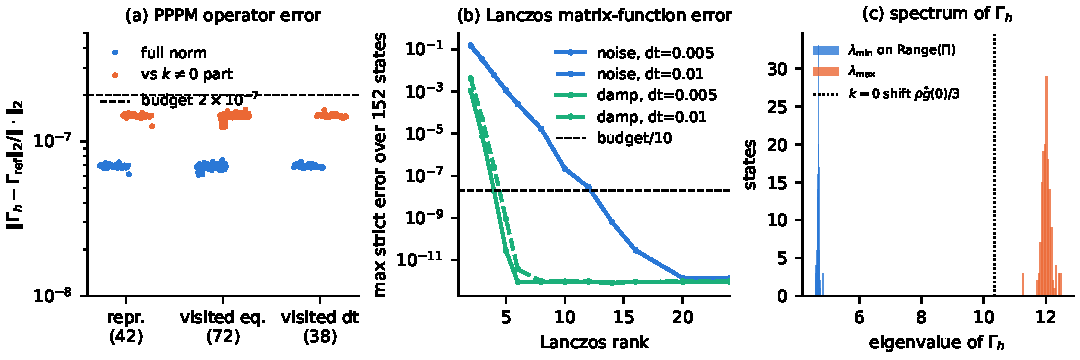
\includegraphics[width=\textwidth]{fig_operator_lanczos.pdf}
\caption{Static verification, LJ+A, $N=256$, $\rho^*=0.75$, $\kT=1$, PPPM $\xi=0.85$, $s_\ast=4.1$, $p=8$, $M=24$;
152 configurations (42 representative, 72 equilibration-visited, 38 dt/long-D-visited); no error bars (each point is
one configuration). (a) Spectral operator error $\eop$ against the full-periodic lattice-sum matrix, full norm and
relative to the $k\neq0$ part; dashed: budget. (b) Lanczos ``strict'' error, i.e.\ the maximum over probe types
(overall, $|k|=2\pi/L$ projection, lowest 3 and lowest 12 eigenmodes) and over all 152 states, relative to the exact output $f(\Gh)\bv$ (or to its $k_{\min}$ or low-mode projection for the
component errors), against the dense matrix function of the same $\Gh$; dashed: budget/10. (c) Extreme eigenvalues of $\Gh$ on
$\Ran(\Pi)$; dotted: $k=0$ contribution $\rho\hat g(0)/3=10.35$. Data: \texttt{lj075\_results/verify\_\{representative,visited\_eq,visited\_dt\}\_A.json};
script \texttt{manuscript/scripts/make\_figures.py}.}
\label{fig:operator}
\end{figure}

\paragraph{Lanczos error.}
The Lanczos error is measured against the dense matrix function of the same $\Gh$ on 4 Gaussian and 4 Maxwell vectors,
the actual momentum of the step, the actual noise draw (regenerated from the run's RNG stream for visited equilibration
states), longitudinal and transverse plane waves at $|\bk|=2\pi/L$ and $\sqrt2\,2\pi/L$, and two slow-mode-dominated
vectors. The strict rule requires the maximum of the overall error and of the $k_{\min}$, lowest-3 and lowest-12
components to be $\le$ budget$/10=2\times10^{-8}$. On the representative states rank 12 suffices for the noise; on one
visited state (a melting fcc start at $t=5$) rank 12 gives a $k_{\min}$ component of $2.88\times10^{-8}$, driven by the
transverse (1,1,0) plane wave. The noise rank was therefore raised to 14 (\cref{fig:operator}(b)). At ranks 14/5 the
worst Lanczos error over all 152 states at $\mathrm dt=0.005$ is $6.4\times10^{-10}$ (noise) and
$2.8\times10^{-11}$ (damping). The dt-study runs used 12/5; their on-line monitor on actual inputs (every 200--500 steps; \texttt{dt\_study.json})
never exceeded $1.6\times10^{-10}$ for the noise, $1.6\times10^{-11}$ for damping and $3.5\times10^{-10}$ for the coupling maps (overall
norm); a $k_{\min}$-component maximum of $1.8\times10^{-9}$ for the noise is stated in \texttt{REPORT.md} but is not stored in any
result file. Monitor values for the equilibration and long-D runs are only in the raw (unavailable) output. Replacing $\Gh$ by $\Gref$ in the O-step changes its output by
at most $1.02\times10^{-8}$; the finite-time FDT residual (damping and noise from the same $\Gh$) is $\le5.5\times10^{-11}$.

\paragraph{Physical effect of the operator error.}
Two replicas were run in lock-step with the same noise from the same start, once with the production set and once with
a tighter set ($\eop\le1.6\times10^{-8}$), at $\mathrm dt=0.005$ for 10 time units. The largest differences of time
averages were $5.9\times10^{-5}$ ($T_{\rm kin}$, relative), $1.4\times10^{-5}$ ($U/N$), $1.3\times10^{-4}$ (MSD at
$t=0.5$--$5$) and $4.5\times10^{-4}$ (pressure, absolute). The RMS position difference grew from $10^{-9}$ at $t=0.1$
to $1.0$--$1.6\times10^{-2}$ at $t=10$. With $n=2$ these are observed maxima, not confidence intervals; the growth of the
pathwise difference is not by itself evidence of a bias.

\subsection{Time discretisation}\label{sec:numerics_time}

We separate two questions: (i) at a fixed time step, how far is the fast method (PPPM+Lanczos) from a dense reference;
(ii) for the fast method, how do results depend on $\mathrm dt$.

\paragraph{(i) Fast versus dense at the same dt.}
For LJ+A the only same-dt fast/dense trajectory comparison is the local pilot of \cref{app:pilot}: one canonical state,
one noise path per dt shared by both methods, $t\le1$, dense meaning $\Gref$ with dense eigendecomposition. The RMS velocity
difference at $t=1$ was $7.4\times10^{-8}$ ($\mathrm dt=0.005$) and $7.8\times10^{-8}$ ($\mathrm dt=0.01$) of the RMS velocity,
consistent with the size of the operator error and at least two orders of magnitude above the Lanczos error. This is
a single path pair and supports no statement on statistical equivalence. A statistical fast/dense comparison with
16 paths per state exists only for the earlier $N=64$ double-well system (\cref{app:history}).

\paragraph{(ii) Time-step dependence: design.}
Four levels $\mathrm dt\in\{0.01,0.005,0.0025,0.00125\}$ were integrated in lock-step from the same state to $t_{\rm end}=10$
with the coupling~\eqref{eq:coupling}, for 16 independent canonical starts (\cref{tab:runs}). Analysis is paired by
replica; time averages use $[1,10]$; the VACF uses every native step $t\ge1$ as an origin, with lags on the common $0.01$ grid; the MSD uses all origins with
centre-of-mass motion removed. The acceptance criteria were committed (commit \texttt{91e20d4}) before the dt-study results were committed
(\texttt{df43e2d}); that no run preceded the criteria is recorded only in the commit message: 1\% relative for $T_{\rm kin}$, $U/N$, the RDF first-peak height and position and MSD at
$t=0.1,0.5,1,2,5$; $0.0075$ absolute for pressure; $E_g\le1\%$ for the RDF ($w=4\pi\rho r^2\dd r$ on $[0.5,L/2)$);
$\max_{t\le2}|\Delta C|/C_{\rm ref}(0)\le1\%$ for the VACF. PASS means the entire 95\% interval lies inside the band, FAIL
that it lies entirely outside, otherwise INCONCLUSIVE. The rule was: compare the finest two levels first, then accept the
largest $\mathrm dt$ whose criteria all PASS. One amendment was made before any multi-replica analysis (Student-$t$ instead of
bootstrap bounds for function-valued criteria). Only after the results were in (commit \texttt{80f8191}) was it found that for
the RDF norm the amended (debiased jackknife) bound is less strict; the registered bootstrap verdict is therefore the one used in
the decision, although \texttt{dt\_study.json} stores the amended verdict (PASS at 0.005). A Bonferroni family-wise view over 36 tests was added
after an interim look and is secondary.

\begin{table}[t]
\centering\small
\caption{Pre-registered dt comparison against $\mathrm{dt}=0.00125$ (16 coupled replicas; mean [95\% paired Student-$t$ CI];
relative unless stated). RDF $E_g$ rows give one-sided 95\% upper bounds; the VACF row gives the maximum over $t\le2$ of
pointwise lower and upper bounds, not a simultaneous band. P/I/F = PASS/INCONCLUSIVE/FAIL. Source: \texttt{lj075\_results/dt\_study.json}, \texttt{summary\_tables.md}.}
\label{tab:dt}
\resizebox{\textwidth}{!}{\begin{tabular}{lccc}
\toprule
criterion & 0.0025 & 0.005 & 0.01 \\
\midrule
$T_{\rm kin}$ & $-0.11\%$ $[-0.32,+0.09]$ P & $-0.12\%$ $[-0.30,+0.07]$ P & $-0.52\%$ $[-0.78,-0.26]$ P \\
$U/N$ & $-0.12\%$ $[-0.23,-0.01]$ P & $-0.05\%$ $[-0.14,+0.04]$ P & $-0.16\%$ $[-0.29,-0.03]$ P \\
pressure (abs.) & $-0.026$ $[-0.049,-0.003]$ I & $+0.0006$ $[-0.018,+0.019]$ I & $-0.024$ $[-0.050,+0.002]$ I \\
RDF $E_g$, registered bootstrap bound & $1.78\%$ I & $1.68\%$ I & $1.82\%$ I \\
RDF $E_g$, debiased jackknife bound & $1.02\%$ I & $0.98\%$ P & $1.02\%$ I \\
RDF first-peak height & $+0.01\%$ $[-0.44,+0.47]$ P & $-0.05\%$ $[-0.50,+0.41]$ P & $+0.02\%$ $[-0.60,+0.64]$ P \\
RDF first-peak position & $+0.03\%$ $[-0.22,+0.28]$ P & $0.00\%$ $[-0.23,+0.22]$ P & $-0.04\%$ $[-0.23,+0.16]$ P \\
VACF $E_V$ [lower, upper] & $[0,0.39\%]$ P & $[0.004\%,0.41\%]$ P & $[0.26\%,0.78\%]$ P \\
MSD(0.1) & $-0.03\%$ $[-0.28,+0.22]$ P & $+0.04\%$ $[-0.19,+0.27]$ P & $+0.14\%$ $[-0.20,+0.48]$ P \\
MSD(0.5) & $+0.13\%$ $[-0.23,+0.50]$ P & $+0.41\%$ $[-0.36,+1.18]$ I & $+0.47\%$ $[-0.45,+1.40]$ I \\
MSD(1) & $+0.25\%$ $[-0.40,+0.90]$ P & $+0.52\%$ $[-0.63,+1.67]$ I & $+0.87\%$ $[-0.54,+2.28]$ I \\
MSD(2) & $+0.69\%$ $[-0.59,+1.98]$ I & $+0.89\%$ $[-1.08,+2.85]$ I & $+1.80\%$ $[-0.15,+3.75]$ I \\
MSD(5) & $+3.44\%$ $[+1.03,+5.86]$ \textbf{F} & $+3.08\%$ $[-0.20,+6.36]$ I & $+2.99\%$ $[-0.32,+6.31]$ I \\
\bottomrule
\end{tabular}}
\end{table}

\begin{figure}[t]
\centering
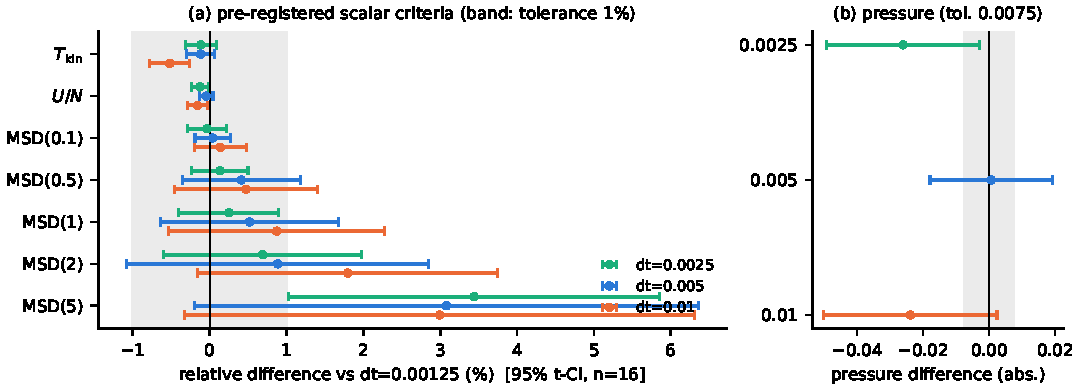
\includegraphics[width=\textwidth]{fig_dt_forest.pdf}
\caption{Pre-registered scalar dt criteria, LJ+A, $N=256$; each level against $\mathrm{dt}=0.00125$, 16 coupled replicas
(ranks 12/5, coupling 4), paired 95\% Student-$t$ intervals. Grey bands: registered tolerances. Shown: $T_{\rm kin}$, $U/N$,
pressure, MSD at five times; the VACF and RDF criteria (including the scalar RDF first-peak height and position) are listed in
\cref{tab:dt} only. Data: \texttt{lj075\_results/dt\_study.json}; script
\texttt{manuscript/scripts/make\_figures.py}.}
\label{fig:dtforest}
\end{figure}

\paragraph{(ii) Results and decision.}
\Cref{tab:dt} and \cref{fig:dtforest} give the results. Under the registered rule \emph{no time step is validated} at $n=16$:
the finest-two comparison is not all-PASS (pressure, RDF norm and MSD(2) are INCONCLUSIVE, MSD(5) FAILs), and no coarser level
passes every criterion. On the subset of criteria that are decidable at this sample size (T, U/N, RDF first peak, VACF
for $t\le2$, MSD(0.1)), all three coarse levels PASS; a rule restricted to that subset would pick $\mathrm{dt}=0.01$, but that rule is
post hoc and is not used as validation.

\emph{dt = 0.005 versus 0.01.} At $\mathrm{dt}=0.01$ the biases in $T_{\rm kin}$ ($-0.52\%$) and $U/N$ ($-0.16\%$) are resolved
(intervals exclude zero) though within 1\%, and the VACF point statistic $E_V=0.52\%$ exceeds its sign-flip noise floor
($0.24\%$); its pointwise lower bound is $0.26\%$. At $\mathrm{dt}=0.005$ no interval of $T_{\rm kin}$ or $U/N$ excludes zero, and only the
pointwise VACF lower bound ($0.004\%$) is nonzero. The MSD point estimates at $t=0.5$--2 are larger at 0.01 than at 0.005
but unresolved. We therefore keep $\mathrm{dt}=0.005$ as a \emph{provisional}, precautionary choice and regard
$\mathrm{dt}=0.01$ as acceptable for static averages ($T$, $U/N$, RDF first peak) with the quoted biases. The configuration
file records \texttt{dt\_validated = None}, \texttt{dt\_provisional = 0.005}.

\emph{The MSD(5) FAIL.} The registered verdict for $\mathrm{dt}=0.0025$ is FAIL. A post-hoc diagnostic shows the same $\approx+3\%$
point estimate for every coarse level against 0.00125 (resolved only at 0.0025), while the differences among the coarse levels
are small but not resolved (0.005 vs 0.0025: $-0.35\%$ $[-3.6,+2.9]$; 0.01 vs 0.005: $-0.09\%$ $[-3.6,+3.4]$); these intervals
cannot exclude a 3\% difference. The pattern would be compatible with a fluctuation of the reference level, but this reading is post
hoc, is not established, and does not change the registered verdict.

\emph{Why the intervals are wide.} The median RMS velocity difference against the 0.00125 path is 0.025/0.057/0.12 at $t=1$
and 0.10/0.20/0.40 at $t=2$ (for 0.0025/0.005/0.01), reaching 0.80--0.86 at $t=5$ (\cref{fig:dtstudy} in \cref{app:extra}).
At $t=5$ this is about 60\% of the value $\sqrt{2\kT/m}\approx1.41$ for fully independent velocities, so pairing loses much of
its variance reduction after $t\approx1$--2; a paired-versus-unpaired variance comparison was not made. We do not attribute this
decorrelation to a specific mechanism. Reaching a 1\% verdict would need roughly 25 replicas for MSD(0.5)
and 80 for MSD(1), and resolving the pressure tolerance roughly 60--100.

\paragraph{Long-time diffusion.}
Eleven coupled two-level chains ($\mathrm{dt}=0.005$ and 0.01, 100 time units, frames every 0.01) give windowed MSD diffusion
coefficients (\cref{fig:diffusion}). With a plateau rule fixed before the long runs were analysed (paired relative change between
consecutive windows within $\pm2\%$ over the whole 95\% CI, required for every step up to the longest window), no plateau
is confirmed at either dt. At $\mathrm{dt}=0.005$, $D_{\rm MSD}$ decreases by $1.9\%$ $[1.2,2.7]$ and then $1.1\%$ $[0.2,2.0]$
per window doubling up to $[4,8]$, and later steps have intervals of $\pm1.4$--$2.6\%$. At $\mathrm{dt}=0.01$ the
decreases are $2.0\%$ $[1.3,2.8]$ and $1.6\%$ $[0.8,2.3]$, one later step meets the plateau condition ($+0.16\%$
$[-1.11,+1.42]$) and the last does not ($-0.96\%$ $[-3.41,+1.50]$). The best current estimate is
$D\approx0.0283$--$0.0286$ ($\mathrm{dt}=0.005$, windows $[4,8]$--$[16,32]$, 95\% half-widths $1.4$--$2.4\%$), not a converged
long-time value. The paired dt effect $D(0.01)/D(0.005)-1$ is resolved
only in the shortest window ($+0.80\%$ $[+0.05,+1.55]$).

\begin{figure}[t]
\centering
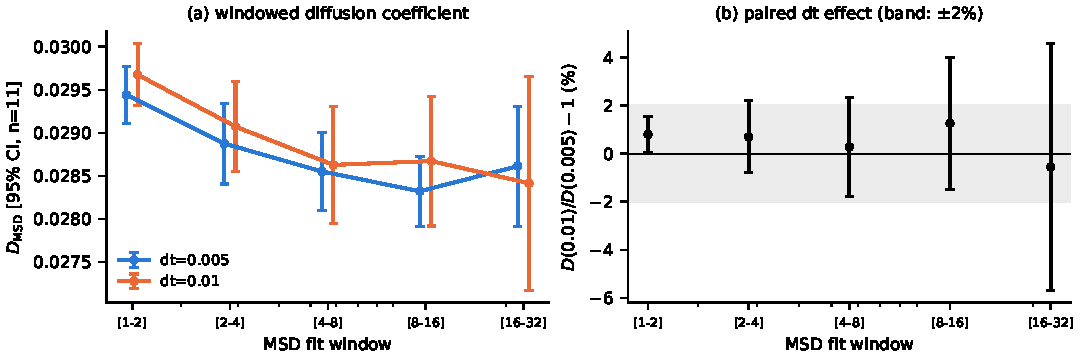
\includegraphics[width=\textwidth]{fig_diffusion.pdf}
\caption{Windowed diffusion coefficient, LJ+A, $N=256$; 11 coupled two-level chains of 100 time units, frames every 0.01,
analysis after $T_0=10$, ranks 12/5. (a) $D_{\rm MSD}$ from linear fits of the MSD on the indicated windows; 95\% Student-$t$
intervals over chains. (b) Paired relative difference between the two time steps, 95\% CI; grey band: $\pm2\%$ for orientation
only (there is no registered dt tolerance for $D$; the $\pm2\%$ plateau rule concerns window-to-window changes). Data: \texttt{lj075\_results/longD.json}; script \texttt{manuscript/scripts/make\_figures.py}.}
\label{fig:diffusion}
\end{figure}

\subsection{Physical observables}\label{sec:numerics_obs}

\paragraph{Static and thermodynamic quantities.}
Eight equilibration runs from four start types (\cref{tab:runs}) give pool means (for $t\ge25$) $U/N=-4.6697$,
$T_{\rm kin}=1.0003$, pressure $0.770$ and RDF first-peak height $2.558$ (\cref{fig:equil} in \cref{app:extra}). The
kinetic temperature is $T_{\rm kin}=\sum_i|\bp_i-\bar\bp|^2/(3m(N-1))$; the pressure is $P=(2K'+W)/(3V)$ with $K'$ the
centre-of-mass-free kinetic energy and $W=-\sum_{i<j}r_{ij}u'(r_{ij})$ the conservative virial (friction and noise do not
enter). A burn-in of 2 time units was measured by a block rule fixed before the analysis (last 2-unit block deviating
by more than $4s_B/\sqrt{n_g}$ from the pool); 5 units are recommended. Start-type dependence after burn-in was not
detected (one-way ANOVA $p=0.21$--$0.78$), but with 2 runs per start type this test has low power, so initial-state
independence is under-sampled, not verified. From the between-run spread, the replicas of 48 time units needed for a 95\%
half-width are 7 ($T_{\rm kin}$ to $\pm0.2\%$), 4 ($U/N$ to $\pm0.2\%$), 4 (RDF peak to $\pm0.5\%$), 10 ($D_{\rm GK}(16)$ to
$\pm5\%$) and 25 (pressure to $\pm0.0075$). The save interval must be one step at $\mathrm{dt}=0.005$ for VACF/Green--Kubo
(quadrature bias $0.23\%$ at $\Delta=0.01$ against a $0.2\%$ rule), whereas the MSD is unaffected up to $\Delta=0.1$
(within $\pm0.1\%$).

\paragraph{Dynamical correlation functions: definitions.}
These follow the project definitions (reproduced to $\le10^{-15}$ on a real trajectory):
\begin{align}
Z(t)&=\frac{\langle\bv_i(t_0)\cdot\bv_i(t_0+t)\rangle}{\langle|\bv|^2\rangle},\qquad
C_b(t)=\frac{\langle\bv_i(t_0)\cdot\bv_j(t_0+t)\rangle_{r_{ij}(t_0)\in b}}{\langle|\bv|^2\rangle},\\
\mathbf j(\bk,t)&=\frac1N\sum_i\bv_i(t)e^{i\bk\cdot\bq_i(t)},\qquad
C_{L}(k,t),\,C_T(k,t)\ \text{from}\ \langle j_{L,T}(\bk,t_0+t)\,j_{L,T}(\bk,t_0)^*\rangle,\\
g_d(r,t)&=\frac{V}{N(N-1)}\Big\langle\sum_{i\neq j}\frac{\delta(r-|\bq_j(t_0+t)-\bq_i(t_0)|_{\rm mi})}{4\pi r^2}\Big\rangle_{t_0},
\end{align}
where $\langle\cdot\rangle_{t_0}$ is the average over time origins, $|\cdot|_{\rm mi}$ the minimum-image distance, and the
$\delta$ function is realised as a histogram divided by the shell volume. Averages without subscript in $Z$, $C_b$ run over
origins and particles (or pairs).
The VCCF shells $b$ are $[0,1.59)$, $[1.59,2.55)$, $[2.55,L/2)$ (first and second minima of $g(r)$). $C_L$, $C_T$ are normalised
mode by mode by their $t=0$ values and averaged over the shells $|\bk|=0.899$ ($k_1$, 3 modes), 1.271 ($k_2$, 6 modes) and
1.798 ($k_4$, 3 modes). $g_d$ is evaluated at $t=0.1,0.5,1,2$; $g_d(r,0)=g(r)$ is shown only. Zero total momentum implies
$\sum_{j\neq i}\bv_i\cdot\bv_j=-|\bv_i|^2$, hence each VCCF bin starts at $-1/(N-1)=-0.00392$ if velocities are independent of
positions; this is not a per-bin baseline and nothing is subtracted.

\paragraph{Sampling.} Two groups of trajectories are analysed separately and never pooled.
The \emph{primary group} is the 16 four-level chains of the dt study: common grid 0.01, lags $\le2$, origins $t_0\in[1,8]$ every
0.05. The \emph{secondary group} is the 11 long-D chains (dt 0.005 and 0.01 only): origins $t_0\in[10,98]$ every 0.25. The
statistical unit is the replica; origins, particles and bins are averaged inside a replica. Curves are normalised by each
level's own $t=0$ value, so these curve verdicts are shape-only, with two exceptions: the ``vacf\_amp'' curve is normalised by
the \emph{reference} level's $C(0)$, and the VCCF is normalised by $\langle|\bv|^2\rangle$, not by $C_b(0)$, so offsets of $C_b(0)$ enter
its differences. Amplitude is otherwise judged through the scalars $C(0)$, $C_L(0)$, $C_T(0)$, whose intervals are per-scalar 97.5\%
paired Student-$t$ intervals over replicas.

\paragraph{Protocol and error definition.}
The protocol was frozen before any difference was computed (v2, commit \texttt{c0434df}) and amended once (v3, commit
\texttt{7484b7d}), also before any difference of the new observables was computed (the protocol itself lists two exceptions that
were not blind: the $C(0)$-scaled VACF and $g(r)$, whose dt differences had been seen in the earlier dt study): every sign lobe of the reference curve is judged on its own. For each
window, $E_{\rm sig}=\sup|\overline{\Delta}|/S$ with $S$ the amplitude of the lobe containing the point; the difference band is
simultaneous at 97.5\% over the window (maximum of a re-studentised sign-flip max-$t$ over all $2^{n-1}$ sign vectors and
Bonferroni-$t$), and the lobe amplitude band is simultaneous at 97.5\%, so both hold jointly at $\ge95\%$. A curve window PASSes
if the upper bound of $E_{\rm sig}$ is $\le1\%$ and every lobe in it is resolved (relative half-width $\le10\%$), FAILs if the lower
bound exceeds 1\%, and is INCONCLUSIVE otherwise. A synthetic self-test of the 95\% band construction gave worst coverage 0.94
(nominal 0.95); the 97.5\% setting and windows with 1--12 points were not covered by the self-test. v2 and v3 differ in 2 of 284
cells, both INCONCLUSIVE$\to$FAIL; we report v3 and list v2 separately in the repository. Pointwise $t$-intervals appear only
in figures.

\begin{figure}[p]
\centering
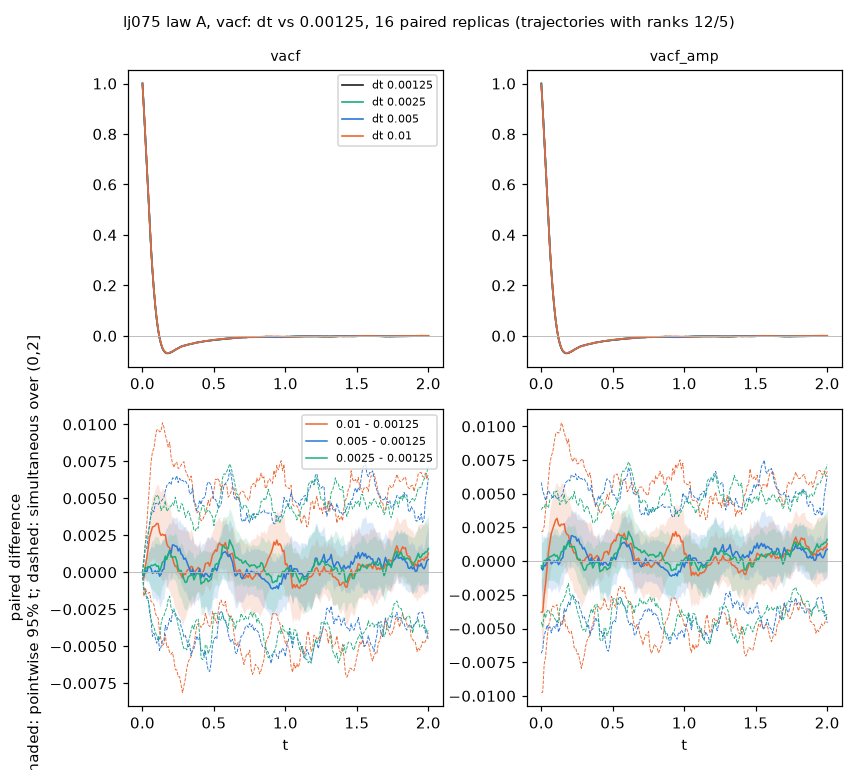
\includegraphics[width=0.62\textwidth]{obs_vacf_primary.png}\\[2pt]
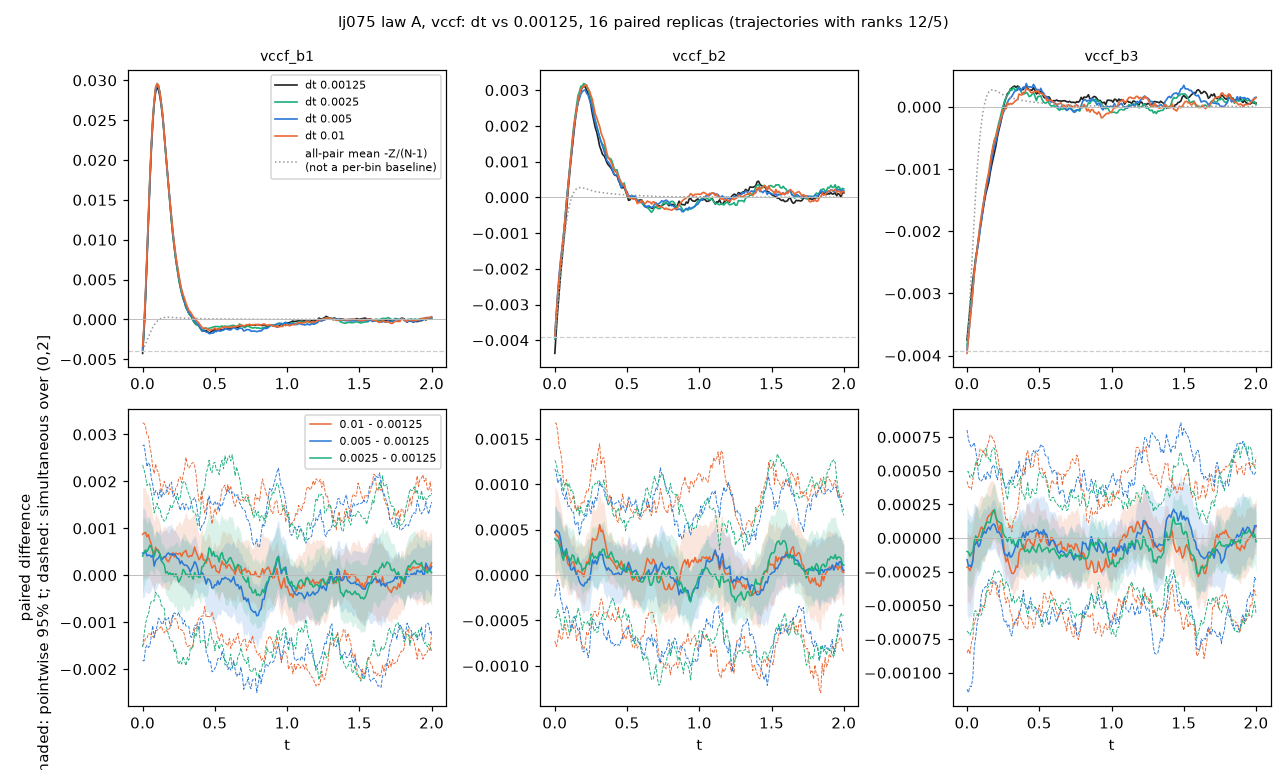
\includegraphics[width=0.92\textwidth]{obs_vccf_primary.png}
\caption{VACF (top; left normalised by each level's $C(0)$, right ``vacf\_amp'' normalised by the reference level's $C(0)$)
and distance-conditioned VCCF $C_b(t)$ for the three shells (bottom), LJ+A, $N=256$, primary group: 16 coupled replicas,
dt $\in\{0.00125,0.0025,0.005,0.01\}$, ranks 12/5, origins $t_0\in[1,8]$. Upper rows: level means. Lower rows: paired differences
against $\mathrm{dt}=0.00125$; shading: pointwise 95\% $t$-interval (not used for verdicts); dashed: simultaneous 97.5\% band of the
whole-curve cell over $(0,2]$. Dotted line in the VCCF panels: all-pair mean $-Z/(N-1)$; light dashed line: $-1/(N-1)$; neither is a per-bin baseline.
Shading uses $n=16$; the dashed band is centred on the mean difference and is also drawn at $t=0$. Source:
\texttt{lj075\_results/observable\_dt/\{vacf,vccf\}\_dt.png}, from \texttt{results.json} (protocol v3).}
\label{fig:vacf_vccf}
\end{figure}

\begin{figure}[p]
\centering
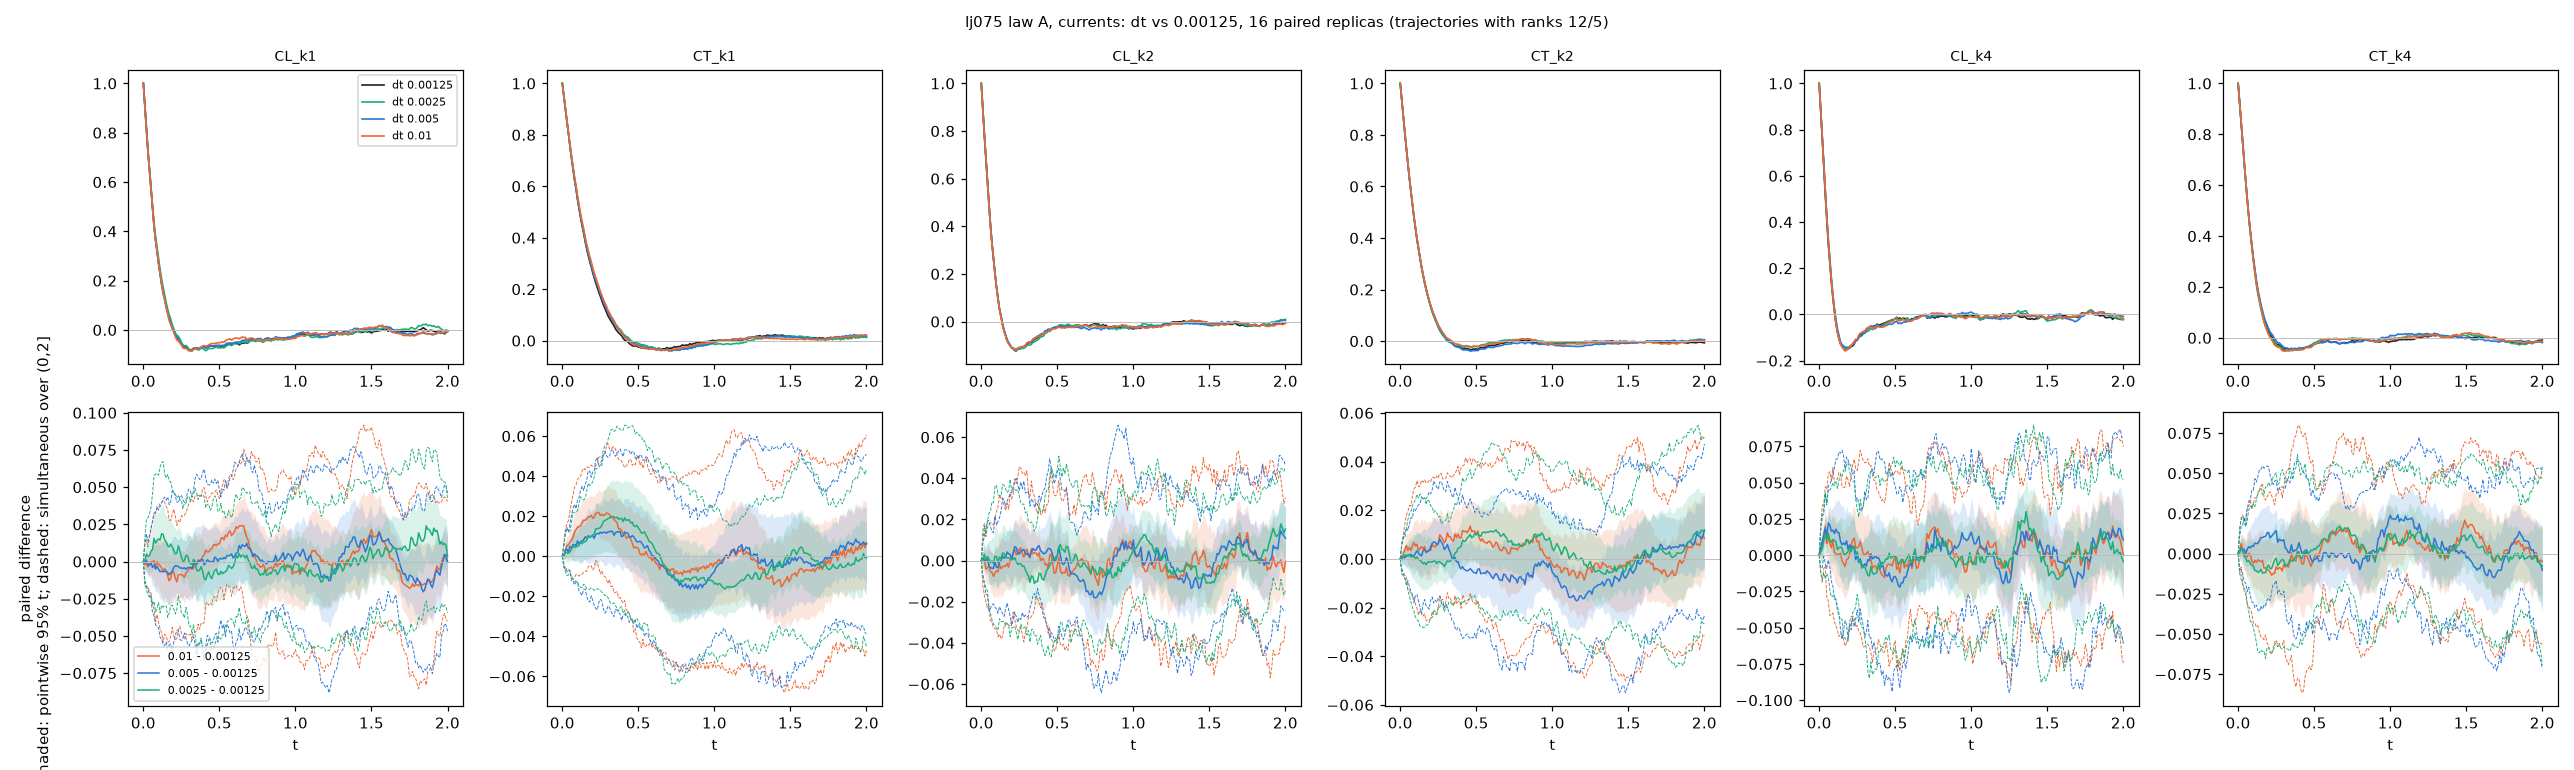
\includegraphics[width=\textwidth]{obs_currents_primary.png}\\[4pt]
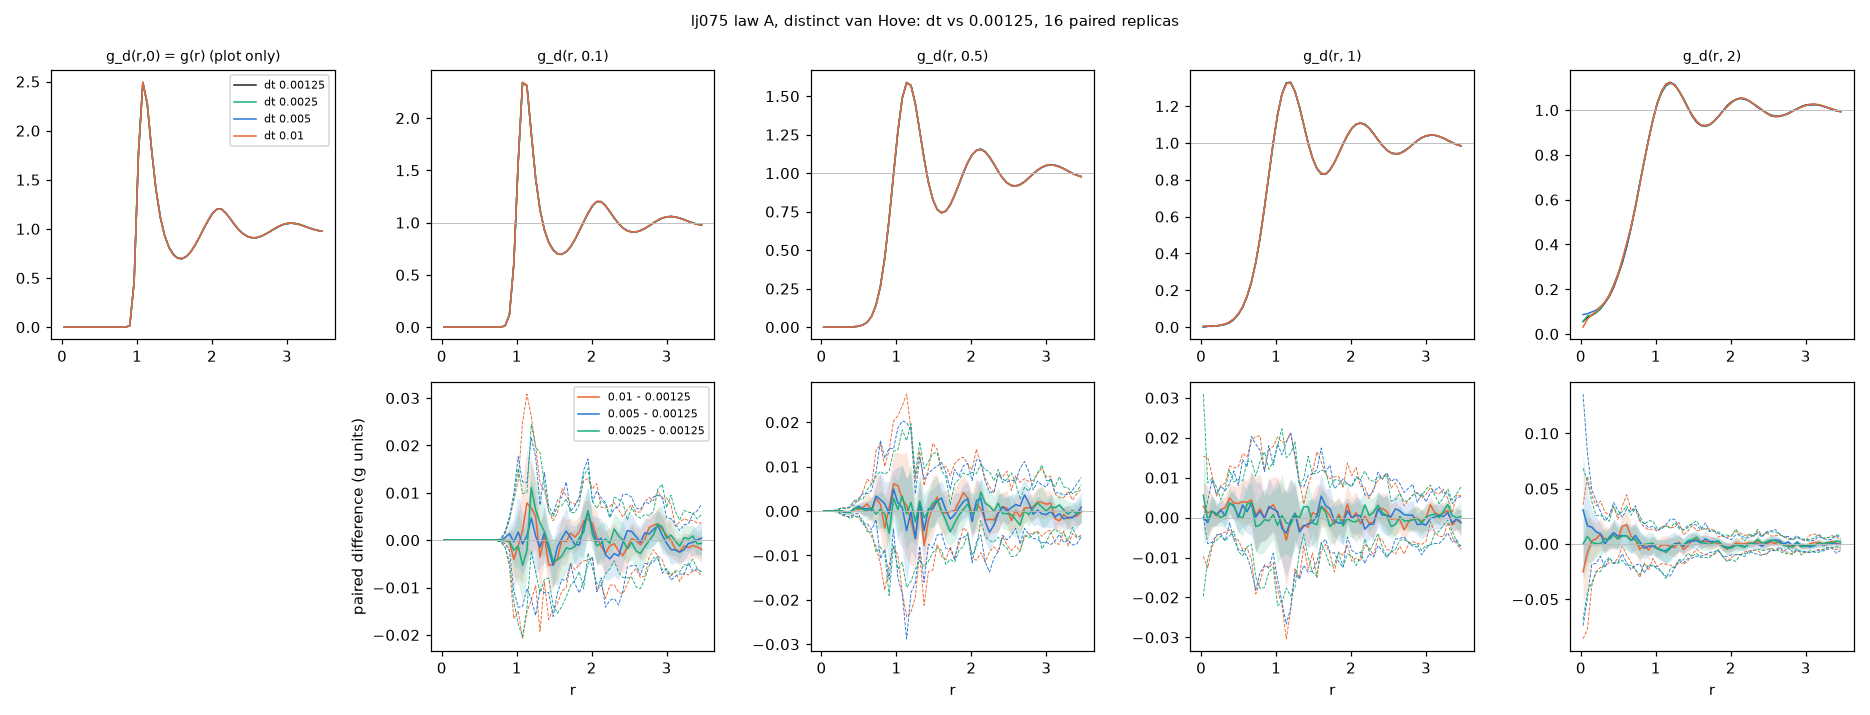
\includegraphics[width=\textwidth]{obs_van_hove_primary.png}
\caption{Top: normalised longitudinal and transverse current correlations $C_L(k,t)$, $C_T(k,t)$ at $|\bk|=0.899$, 1.271,
1.798. Bottom: distinct van Hove function $g_d(r,t)$ at $t=0,0.1,0.5,1,2$ ($t=0$ shown only). Same data, groups, bands and
conventions as \cref{fig:vacf_vccf}. For $g_d$ the dashed band is simultaneous only over $r$ bins with at least 100 reference pairs per
replica (e.g.\ $r>0.79$ at $t=0.1$); it carries no coverage in the excluded small-$r$ bins. Source:
\texttt{lj075\_results/observable\_dt/\{currents,van\_hove\}\_dt.png}.}
\label{fig:currents_vanhove}
\end{figure}

\paragraph{Results.}
\Cref{fig:vacf_vccf,fig:currents_vanhove} show the primary group; the secondary group is in \cref{app:extra}. The main
findings, all at 1\% of each feature's own lobe amplitude, are:
\begin{itemize}
\item \emph{Display support.} Of 71 observable$\times$window cells, a single cell is SUPPORTED for $\mathrm{dt}=0.01$ (and the same for
0.005): the van Hove core window at $t=0.1$, which contains one $r$ bin ($r=0.84$) where $g_d\approx0.012$. It says nothing about
the van Hove structure. Five cells are NOT SUPPORTED because of FAILs; the other 65 are INCONCLUSIVE.
\item \emph{Resolved deviations at dt = 0.01 vs 0.00125.} $\langle|\bv|^2\rangle$ is lower by $0.38\%$ $[0.09,0.67]$ (PASS at
1\%); $C_T(k_1)$ decays more slowly for $t\le0.5$ (half-decay time $+3.6\%$ $[+0.6,+6.6]$); $g_d(r<0.9,t=2)$ differs by
$E_{\rm sig}=1.9\%$ $[0.14,4.6]$. All except $\langle|\bv|^2\rangle$ are INCONCLUSIVE against 1\%. For the $g_d(t=2)$ cell the levels
0.0025 and 0.005 give the same offset, which suggests a low reference mean rather than a dt trend; this is not established.
\item \emph{FAIL cells.} Seven of 284 cells FAIL (5 of 224 window cells, 2 of 60 whole-curve cells), six involving
$\mathrm{dt}=0.01$ and five in the secondary 0.01 vs 0.005 comparison (VCCF far shell for $t\in(0.2,0.5]$; $C_L(k_1)$ for
$t\in(0.5,1]$; $C_L(k_2)$ for $t\in(1,2]$; and the whole-curve cells of the far shell and of $C_L(k_1)$). All lie in windows whose
reference lobes are unresolved. One primary FAIL (0.005 vs 0.00125, VCCF second shell, $t\le0.2$) appears to be driven mainly by an
offset of the shared reference at $t=0$ ($C_b(0)=-0.00437$, 2.5 replica-SE below $-1/(N-1)$, while all three coarser levels lie
$4$--$5\times10^{-4}$ above it). At this sample size the FAIL counts cannot separate chance from a dt
effect; the counts are reported as observed.
\item \emph{No whole-curve deviation is resolved in the primary group; this is not equivalence.} The simultaneous upper bounds at
$\mathrm{dt}=0.01$ are $1.0\times10^{-2}$ of $C(0)$ (VACF), $3.2\times10^{-3}$ of $\langle|\bv|^2\rangle$ (first-shell VCCF), 0.092
($C_L(k_1)$), 0.068 ($C_T(k_1)$) and 0.030/0.045 ($g_d$ at $t=1,2$, in $g$ units). Effects up to these sizes are not excluded.
\item \emph{Why most cells are undecided.} Weak reference lobes (VACF dip in the primary group, negative lobes of $C_L$, $C_T$,
second and third VCCF shells, van Hove tails) are not resolved to $\pm10\%$, so PASS is impossible there; where lobes are resolved,
the difference bands still reach 1.5--8.5\% of the lobe amplitude.
\item \emph{Secondary group, 0.01 vs 0.005.} $D_{\rm GK}$ to $t=2$ PASSes on the protocol's integral scale
$(1/3)\int_0^2|C|\dd t\approx2.3D_{\rm GK}$; relative to $D_{\rm GK}$ itself the difference is $+0.55\%$ $[-0.78,+1.88]$, so 1\%
agreement of $D_{\rm GK}$ is not shown. The VACF zero crossing and the $g_d$ first-peak excess at $t=0.1$ also PASS; these are
agreements between 0.01 and 0.005 only and cannot by themselves confer display support.
\end{itemize}
A decay of a correlation function to zero is not used as evidence that the model is correct, and long-lag differences are not
attributed to chaos or sampling noise without a test that separates them. A burst design for the $t\le0.5$ features (about 170
coupled bursts, 6.8 core-hours) is described in \texttt{followup\_plan.json} and was not run. Its sizing assumes a true difference of
zero, uses the lobe amplitude rather than its lower bound (about 207 rather than 167 bursts for the VACF dip), ignores the lobe-resolution
requirement (the primary VACF dip lobe is unresolved, so that cell cannot PASS by more bursts alone), and grows to about 1000--1650
bursts at the differences observed so far.

\subsection{Cost}\label{sec:numerics_cost}

All LJ+A timings below were recorded on the development virtual machine (host ``vm''; the CPU model, Xeon 2.80\,GHz, is recorded only
for the pilot), single thread (OpenBLAS/OMP/MKL threads = 1). \Cref{tab:cost} reports CPU time per step; the dt comparison and the
pilot report wall-clock step times. We do
not combine them with timings from other machines, and queue or scheduling time never enters.

\paragraph{Production step.}
The median CPU time of one full BAOAB step (forces, $\Gh$ build, Lanczos damping and noise) at $\mathrm{dt}=0.005$, from 6
interleaved rounds of 40 steps, is given in \cref{tab:cost}. Raising the noise rank from 12 to 14 costs $+8\%$. At ranks 14/5,
one time unit costs $0.0075$ core-hours at $\mathrm{dt}=0.005$.

\begin{table}[t]
\centering\small
\caption{Production-step cost, LJ+A, $N=256$, single thread, $\mathrm{dt}=0.005$ (\texttt{lj075\_results/pppm\_cost.json}).}
\label{tab:cost}
\resizebox{\textwidth}{!}{\begin{tabular}{lcccc}
\toprule
PPPM set & ranks & max $\eop$ (verification set)$^{a}$ & ms/step, median [min, max] & core-h per time unit \\
\midrule
$\eta$ 0.6779, $p$ 8 (production) & 12/5 & $7.3\times10^{-8}$ & 124.8 [122.4, 130.1] & 0.0069 \\
$\eta$ 0.6779, $p$ 8 (production) & 14/5 & $7.6\times10^{-8}$ & 134.9 [133.2, 136.8] & 0.0075 \\
$\eta$ 0.6, $p$ 7 & 12/5 & $7.6\times10^{-8}$ & 117.9 [113.4, 124.8] & 0.0065 \\
$s_\ast$ 4.4, $\eta$ 0.6, $p$ 7 & 12/5 & $1.6\times10^{-8}$ & 140.0 [132.4, 155.6] & 0.0078 \\
\bottomrule
\end{tabular}}
\par\smallskip\raggedright\footnotesize $^{a}$ The two production rows differ only in the state set used for verification
(representative for 12/5, equilibration-visited for 14/5), not in the operator.
\end{table}

\paragraph{dt = 0.01 versus 0.005.}
In a separate session of interleaved production-runner runs (3 rounds of 300 steps per setting, no frame output), the median
per-step cost differed by at most 2.6\% between the two step sizes, and the measured saving per physical time of
$\mathrm{dt}=0.01$ over 0.005 was $48.7\%$ (ranks 12/5) and $50.4\%$ (14/5), consistent with the 50\% step-count estimate.
These per-step times (0.18--0.20 s) differ from \cref{tab:cost} because they include the production runner's overhead;
the two measurements are not mixed.

\paragraph{Fast versus dense at matched model.}
The local pilot (\cref{app:pilot}) timed both O-steps for the same model and state on the same machine, in the same session:
median integration-step time $0.208$ s (fast, PPPM + Lanczos 14/5) versus $1.129$ s (dense $\Gref$ with eigendecomposition) at
$\mathrm{dt}=0.005$, and $0.204$ versus $1.034$ s at $\mathrm{dt}=0.01$; peak resident memory 121 MB versus 604 MB. The accuracy is not
matched in the strict sense: the dense step is the model ($\eop\approx0$; lattice-sum truncation $\sim10^{-11}$ per pair), the fast step carries $\eop\approx7\times10^{-8}$. The dense step
times varied strongly (90th percentile 2.3--2.5 times the median), for reasons not investigated. A same-model comparison of dense,
direct-sum and PPPM with operator construction, single $\Gamma\bv$ and full step timed separately, at matched accuracy and over
$N=64$--1728, exists only for the earlier toy state point (\cref{app:history}); a size scan at the LJ+A state point has not been run.

\subsection{Reproducibility and data scope}\label{sec:repro}

Every result file carries a provenance block (command, git commit, dirty flag, script hashes, library versions, thread
settings). Raw trajectories of the LJ+A study (\texttt{lj075\_results/raw/}) are git-ignored and are \emph{not} available in the
repository clone used for this draft; their SHA-256 hashes are recorded in \texttt{observable\_dt/inventory.json}. Consequently:
the figures and tables of this paper can be regenerated from cached analysis files (JSON, \texttt{per\_replica\_observables.npz});
any new observable, a different window or a different statistical protocol on the existing trajectories requires the raw files,
which must be retrieved from the machine that produced them \todo{location of raw LJ+A trajectories}. The same holds for the toy
trajectories of \cref{app:history} (manifest lists 76 files, 413.8 MB, absent). See \texttt{evidence\_map.md} for a per-item list.

%======================================================================
\section{Discussion and limitations}\label{sec:discussion}
%======================================================================

\paragraph{What is established for LJ+A at $\rho^*=0.75$, $\kT=1$, $N=256$.}
(a) The structural properties of the model (symmetry, positivity, momentum null space, FDT and invariance of the Gibbs measure)
hold for the continuous model and, except positivity, for the PPPM matrix by construction. (b) The PPPM operator meets the
$2\times10^{-7}$ budget against the full-periodic lattice-sum matrix on 152 static and visited configurations, and positivity on
$\Ran\Pi$ holds on all of them. (c) Lanczos ranks 14/5 meet a strict error rule ($\le2\times10^{-8}$) on all 152 states, with
worst error $6.4\times10^{-10}$. (d) Momentum is carried to round-off. (e) The effect of the operator error on time averages
was $\le1.3\times10^{-4}$ relative in two lock-step replicas. (f) $T$, $U/N$, the RDF first peak, the VACF for $t\le2$ and MSD(0.1)
PASS the registered 1\% criteria at all of $\mathrm{dt}=0.0025$, 0.005 and 0.01.

\paragraph{What is provisional or under-sampled.}
No time step is validated under the registered rule; $\mathrm{dt}=0.005$ is provisional. The dt effect on the RDF norm, on MSD
at $t\ge0.5$, on pressure and on the long-time diffusion coefficient is unresolved at $n=16$ and $n=11$. The long-time $D$ has no
confirmed plateau at the $\pm2\%$ level. Initial-state independence after burn-in is not verified (2 runs per start type). Most
comparisons of the dynamical correlation functions at 1\% of lobe amplitude are INCONCLUSIVE; several resolved deviations at
$\mathrm{dt}=0.01$ (kinetic temperature, transverse current at $k_1$) and seven FAIL cells are reported as observed without a
mechanism. The dynamic runs used ranks 12/5, below the later recommendation 14/5; the on-line Lanczos monitor of the dt-study runs stayed below
$4\times10^{-10}$ (overall norm); the equilibration and long-D monitors are not available.

\paragraph{What is not addressed.}
No size scan at the LJ+A state point (only $N=256$), so the $O(N\log N)$ scaling is supported only by earlier toy and ideal-gas
tests at fixed rank (\cref{app:history}); on frozen random $\kappa=1$ configurations the adaptive-tolerance rank grew as $N^{0.34}$. No weak-order or strong-order
convergence theorem is proved for the scheme with configuration-dependent matrix friction and Lanczos noise; the stationary
distribution of the discrete scheme is not characterised. The influence function is not optimised. The cheaper PPPM alternative
of \cref{tab:operator} is verified statically only. No HPC run has been performed: the HPC scripts were exercised by local
emulation only (\cref{app:pilot}). Kernel B was stopped before analysis. There is no external validation against molecular dynamics
or experiment, and no reproduction of Ref.~\cite{LyuLei2023} is claimed.

\paragraph{Next steps implied by the data.}
About 25 replicas for MSD(0.5) and 60--100 for pressure at 1\%; about 16--60 runs of 100 time units to confirm a $\pm2\%$ plateau of
$D$; about 170 coupled short bursts for the $t\le0.5$ correlation features; a size scan with the 14/5 configuration; the cluster
pilot. None of these were run for this draft.

\appendix

%======================================================================
\section{Proofs and closed forms}\label{app:proofs}
%======================================================================

\subsection{Closed form of $\rho_\kappa$}
With $a=\kappa^2/4$,
\[\frac{\dd}{\dd s}\Big[2\sqrt{\tfrac{s}{\pi}}\,e^{-a/s}\Big]=w_\kappa(s)+\frac{\kappa^2}{2\sqrt\pi}s^{-3/2}e^{-a/s},\qquad
\frac{\dd}{\dd s}\Big[-\kappa\erfc\Big(\frac{\kappa}{2\sqrt s}\Big)\Big]=-\frac{\kappa^2}{2\sqrt\pi}s^{-3/2}e^{-a/s}.\] The sum is $w_\kappa$; both
terms vanish as $s\to0^+$. Positivity follows from $\rho_\kappa=\int_0^sw_\kappa>0$. For numerical stability the code evaluates the
algebraically identical form $\rho_\kappa=\frac{2\sqrt s}{\sqrt\pi}e^{-a/s}\,p(\kappa/(2\sqrt s))$, $p(x)=1-\sqrt\pi x\,\mathrm{erfcx}(x)$,
and checks it against the literal expression.

\subsection{Hessian representation and $E_1$ closed forms}\label{app:hessian}
For each $s>0$, $\partial_i\partial_je^{-sr^2}=(4s^2x_ix_j-2s\delta_{ij})e^{-sr^2}$, hence
$x_ix_je^{-sr^2}=\frac{1}{4s^2}\partial_i\partial_je^{-sr^2}+\frac{\delta_{ij}}{2s}e^{-sr^2}$. Multiplying by $\rho_\kappa(s)$ and
integrating over any $s$-interval $I$ gives $\br\br^{\mathsf T}\int_I\rho_\kappa e^{-sr^2}=\nabla\nabla\varphi_I+\psi_I\Id$ with
the restricted integrals; differentiation under the integral is justified for $r>0$ since $\rho_\kappa(s)/s^2=O(s^{-3/2})$ at infinity
and $O(s^{-1/2}e^{-\kappa^2/4s})$ at zero. For $I=(0,\infty)$:
$\partial_{(r^2)}\psi_\kappa=-\frac12\int\rho_\kappa e^{-sr^2}=-\frac{e^{-\kappa r}}{2r^3}$, so $\psi_\kappa'(r)=-e^{-\kappa r}/r^2$ and,
with $\psi_\kappa(\infty)=0$, $\psi_\kappa(r)=\int_r^\infty e^{-\kappa t}t^{-2}\dd t=e^{-\kappa r}/r-\kappa E_1(\kappa r)$. Similarly
$\varphi_\kappa'(r)=-r\psi_\kappa(r)$, and using $\int uE_1(u)\dd u=\frac{u^2}{2}E_1(u)-\frac{(u+1)e^{-u}}{2}$,
$\varphi_\kappa(r)=\int_r^\infty t\psi_\kappa(t)\dd t=\frac{1}{2\kappa}[(1-x)e^{-x}+x^2E_1(x)]$, $x=\kappa r$. Note
$\varphi_\kappa(0)=1/(2\kappa)$ is finite while $\psi_\kappa(r)\sim 1/r$ as $r\to0$. Numerical checks: see
\cref{rem:hessian} (script \texttt{manuscript/scripts/verify\_closed\_forms.py}).

\subsection{Fourier transform of the full kernel}\label{app:fourier_full}
By isotropy, $\hat K_\kappa(\bk)=a(k)\Id+b(k)\kh\kh^{\mathsf T}$ with $3a+b=\int e^{-i\bk\cdot\br}e^{-\kappa r}/r\dd\br=4\pi/(k^2+\kappa^2)$.
The transverse part is $a(k)=4\pi\int_0^\infty re^{-\kappa r}\frac{j_1(kr)}{kr}\dd r=\frac{4\pi}{k^3}I(k)$ with
$I(k)=\int_0^\infty e^{-\kappa r}\frac{\sin kr-kr\cos kr}{r^2}\dd r$. Differentiating, $I'(k)=k\int_0^\infty e^{-\kappa r}\sin kr\dd r=\frac{k^2}{k^2+\kappa^2}$,
$I(0)=0$, so $I(k)=k-\kappa\arctan(k/\kappa)$. Thus~\eqref{eq:Kfull_fourier} with $\lambda_\parallel=a+b=4\pi/(k^2+\kappa^2)-2a$. As
$k\to0$, $a\to4\pi/(3\kappa^2)$, consistent with~\eqref{eq:k0}. Numerical check against radial quadrature at
$k\in\{0.05,0.9,1.3,4\}$, $\kappa=0.7$: relative error $\le7.2\times10^{-10}$.

\subsection{Stationarity of the Gibbs measure}
See the proof of \cref{prop:invariance}; the friction part of the Fokker--Planck operator is
$\mathcal L^*_{\rm fr}\pi=\nabla_{\bp}\cdot\big[\Gamma(\bq)\big(\tfrac{\bp}{m}\pi+\kT\nabla_{\bp}\pi\big)\big]$, which vanishes for
$\pi\propto e^{-|\bp|^2/(2m\kT)}$. This is the same mechanism as in dissipative particle dynamics~\cite{EspanolWarren1995}.

%======================================================================
\section{Additional figures for the LJ+A study}\label{app:extra}
%======================================================================

\begin{figure}[htbp]
\centering
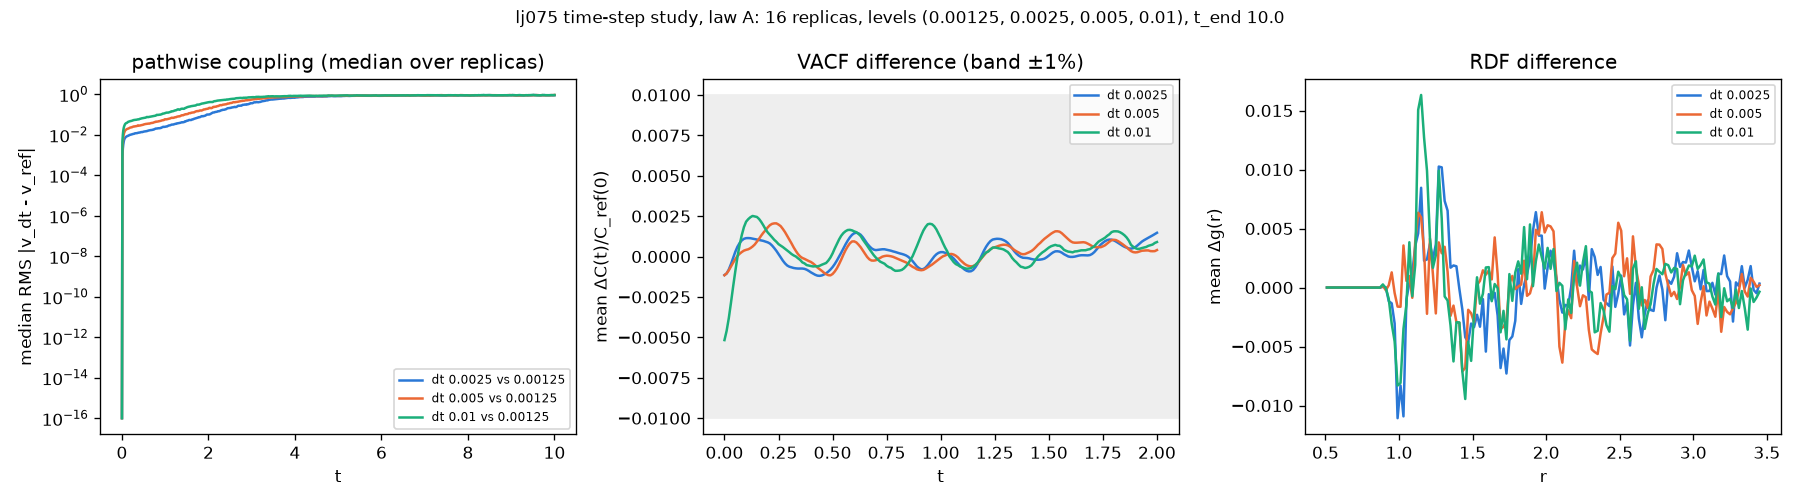
\includegraphics[width=\textwidth]{dt_study_A.png}
\caption{dt study, LJ+A, 16 coupled replicas, levels 0.00125--0.01, $t_{\rm end}=10$, ranks 12/5. Left: median over replicas of the
RMS velocity difference to the 0.00125 path. Middle: mean VACF difference (grey: $\pm1\%$ band). Right: mean RDF difference. Middle
and right panels show means only, without intervals; verdicts use \cref{tab:dt}. Source: \texttt{lj075\_results/dt\_study\_A.png}.}
\label{fig:dtstudy}
\end{figure}

\begin{figure}[htbp]
\centering
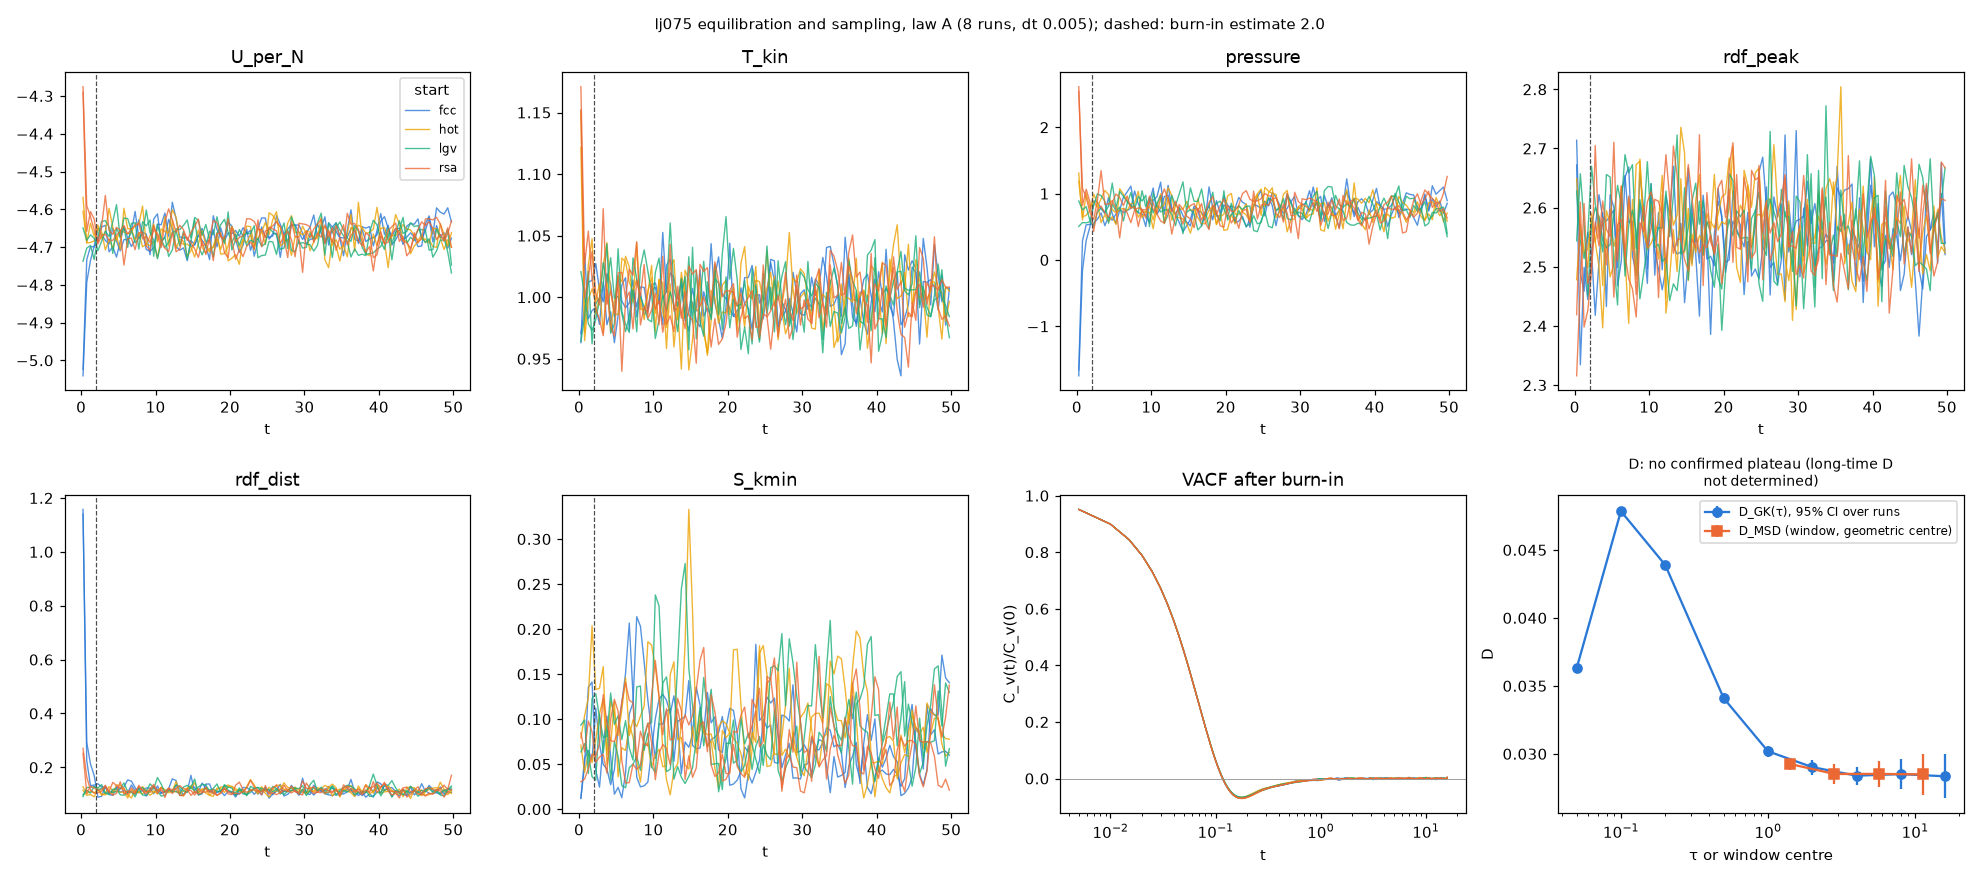
\includegraphics[width=\textwidth]{equilibration_A.png}
\caption{Equilibration, LJ+A, 8 runs of 50 time units at $\mathrm{dt}=0.005$ (ranks 12/5), four start types (two runs each); dashed line:
measured burn-in 2.0. Bottom right: $D_{\rm GK}(\tau)$ and windowed $D_{\rm MSD}$ with 95\% CIs over the 8 runs; no plateau is confirmed.
Source: \texttt{lj075\_results/equilibration\_A.png}.}
\label{fig:equil}
\end{figure}

\begin{figure}[p]
\centering
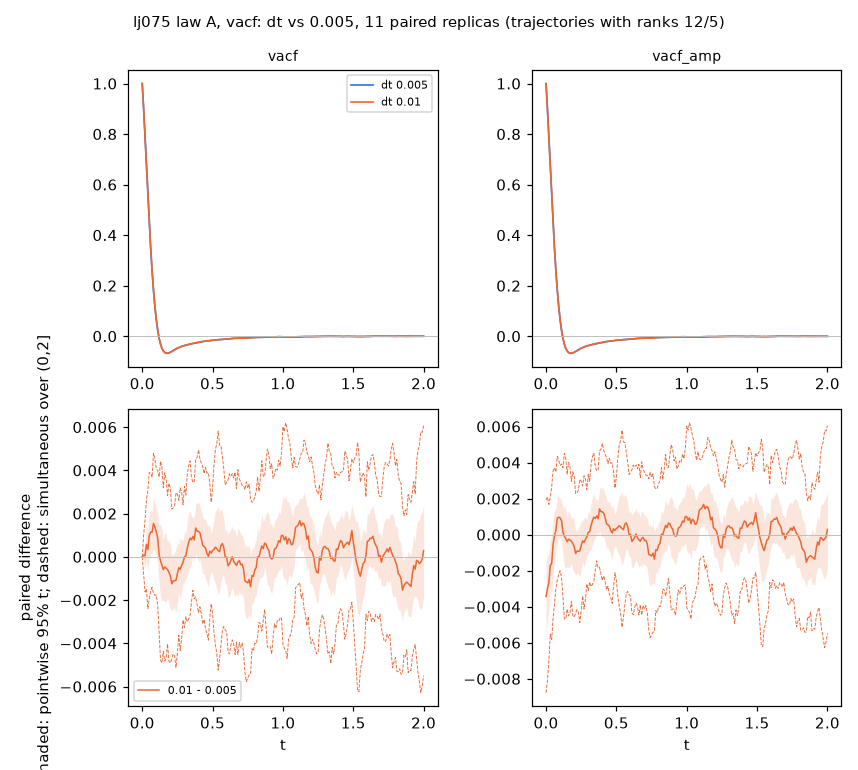
\includegraphics[width=0.55\textwidth]{obs_vacf_secondary.png}\\
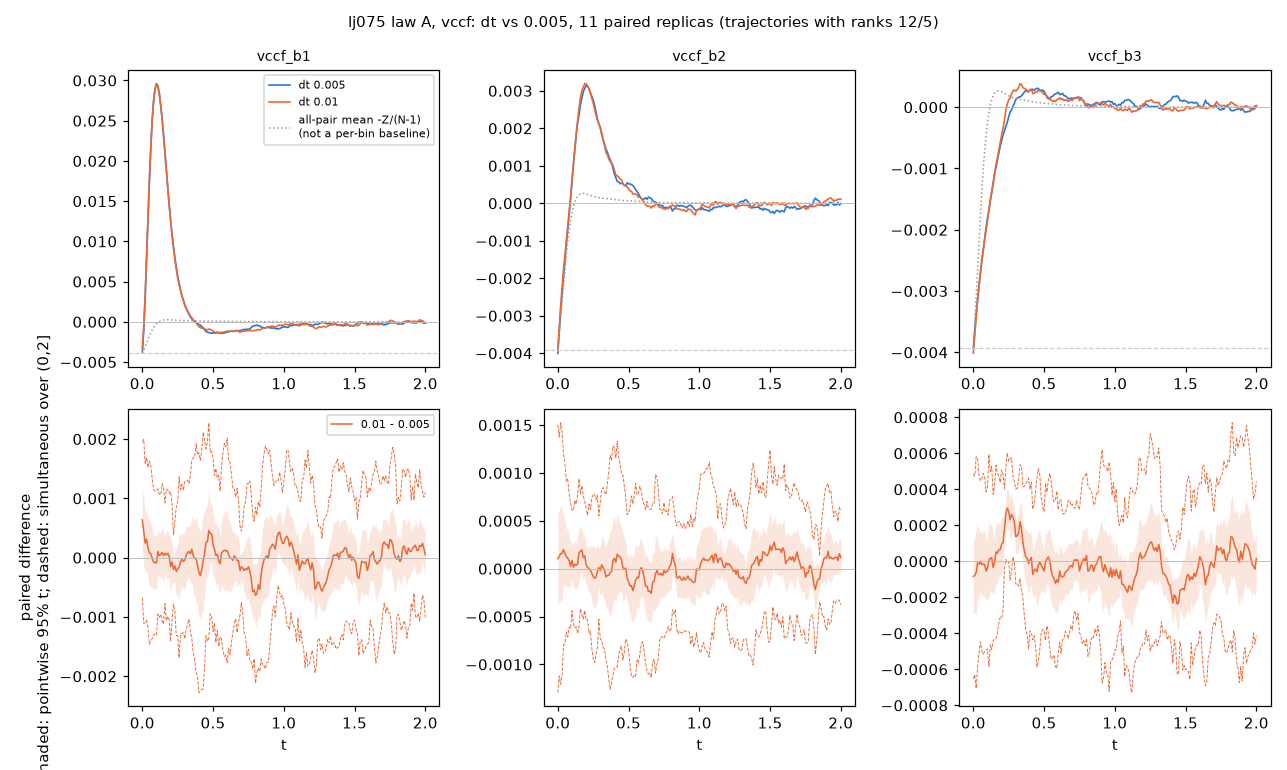
\includegraphics[width=0.85\textwidth]{obs_vccf_secondary.png}
\caption{Secondary group, VACF and VCCF: 11 coupled two-level chains, $\mathrm{dt}=0.01$ versus 0.005 only, origins
$t_0\in[10,98]$ every 0.25, ranks 12/5. Same layout and band conventions as \cref{fig:vacf_vccf}. This group holds five of the
seven FAIL cells; it cannot confer display support because it has no finer reference level. Source:
\texttt{lj075\_results/observable\_dt/\{vacf,vccf\}\_dt\_secondary.png} (drawn from stored means and paired differences in
\texttt{results.json}).}
\label{fig:secondary}
\end{figure}

\begin{figure}[p]
\centering
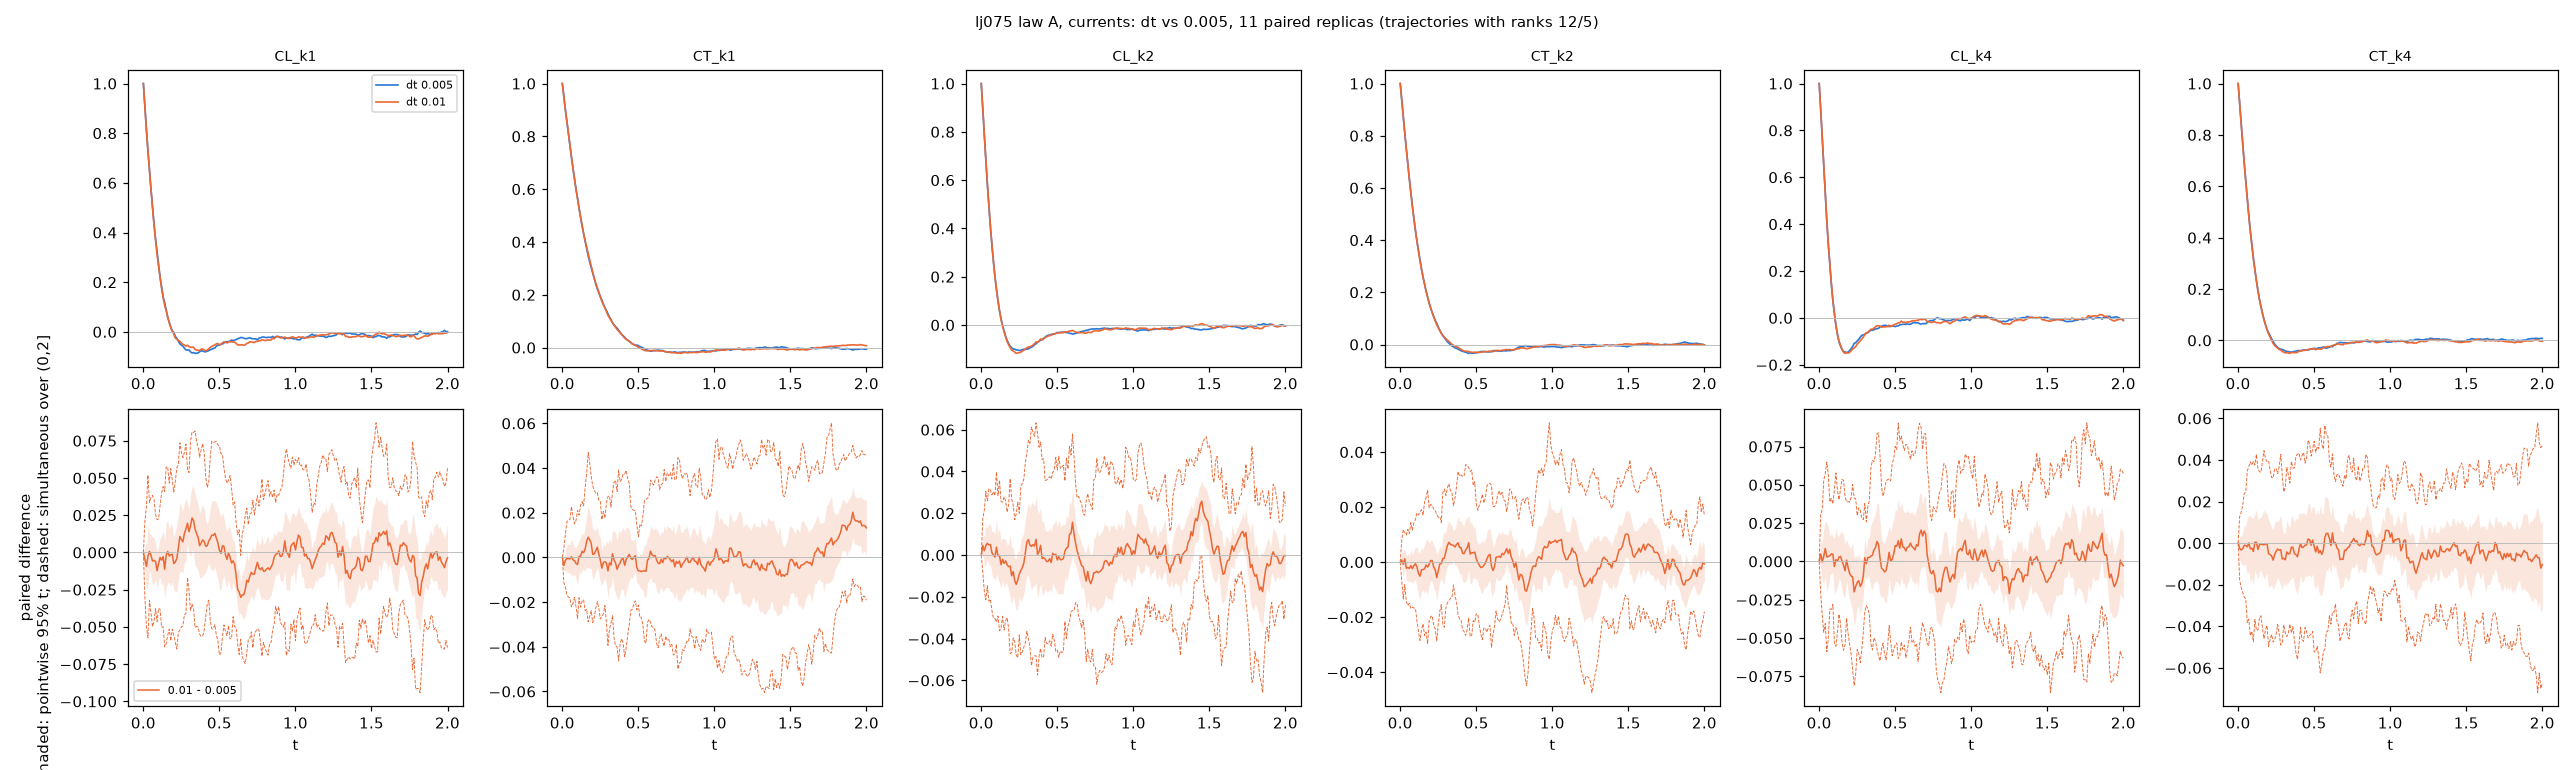
\includegraphics[width=\textwidth]{obs_currents_secondary.png}\\[4pt]
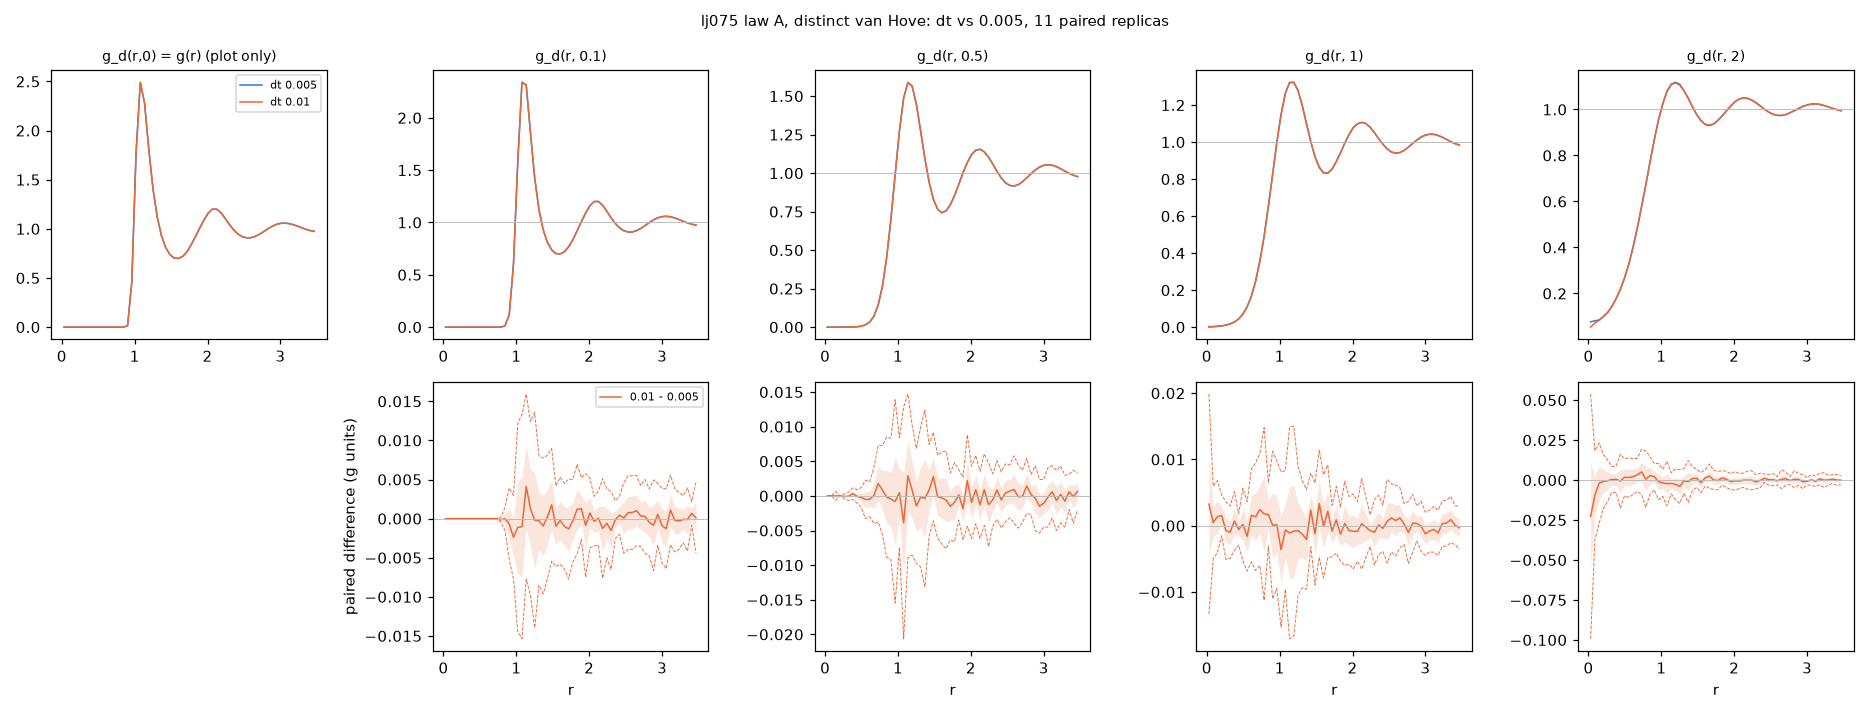
\includegraphics[width=\textwidth]{obs_van_hove_secondary.png}
\caption{Secondary group, current correlations and distinct van Hove function; data and conventions as in \cref{fig:secondary}
and \cref{fig:currents_vanhove}. Source: \texttt{lj075\_results/observable\_dt/\{currents,van\_hove\}\_dt\_secondary.png}.}
\label{fig:secondary2}
\end{figure}

\clearpage
%======================================================================
\section{Local emulation of the HPC pilot}\label{app:pilot}
%======================================================================

The HPC workflow (Slurm scripts, checkpoint/restart, locking) was exercised \emph{locally} with bash on the development VM, without
Slurm (\texttt{hpc\_pilot/local\_20261010}; \texttt{on\_slurm=false}, no job IDs). It is \emph{not} a cluster result, and no newer
cluster result exists in the repository. Setup: configuration \texttt{lj\_rho0.75\_kT1.0\_A\_prod}; fast O-step = PPPM + Lanczos 14/5;
dense O-step = $\Gref$ with dense eigendecomposition; $\mathrm{dt}=0.005$ (200 steps) and 0.01 (100 steps) to $t=1$; one initial state
(step 10000 of equilibration run s305, which used ranks 12/5); fast and dense share the noise at each dt; the two dt values are not
coupled; one thread.

All workflow checks passed (three-segment restart bitwise equal to a continuous twin, lock refusal, checkpoint cadence, every-step
frames; Lanczos monitor self-estimate below $4.9\times10^{-11}$ against the budget $2\times10^{-7}$). Fast$-$dense differences at $t=1$: RMS
position $1.96\times10^{-8}$/$2.22\times10^{-8}$, RMS velocity $1.28\times10^{-7}$/$1.35\times10^{-7}$
($7.4\times10^{-8}$/$7.8\times10^{-8}$ of the RMS velocity) for $\mathrm{dt}=0.005$/0.01; $\max_t|\Delta T_{\rm kin}|\le1.3\times10^{-8}$.
$|P(t)-P(0)|\le1.3\times10^{-13}$ in all four cases. The difference is dominated by the PPPM operator error (relative Frobenius
$4.1$--$4.3\times10^{-8}$), not by Lanczos truncation. Fitted growth rates of the differences over $[0.1,1]$ (1.45--2.42) are fits,
not Lyapunov exponents. The value $4.9\times10^{-11}$ is the maximum of the run monitor's self-estimates
$\|f_r-f_{r+e}\|/\|f_{r+e}\|$ over four columns (noise and damping, full and $k_{\min}$-projected; \texttt{toy\_run.MON\_COLS});
which column attains it cannot be recovered because the raw monitor files are not in the repository. The actual noise-function Lanczos
error, against the dense matrix function of the same $\Gh$ on the monitor's own random input, is $\le4.3\times10^{-12}$ (damping
$\le1.5\times10^{-11}$; \texttt{pilot\_results.json}, key \texttt{lanczos\_check}).

\begin{figure}[htbp]
\centering
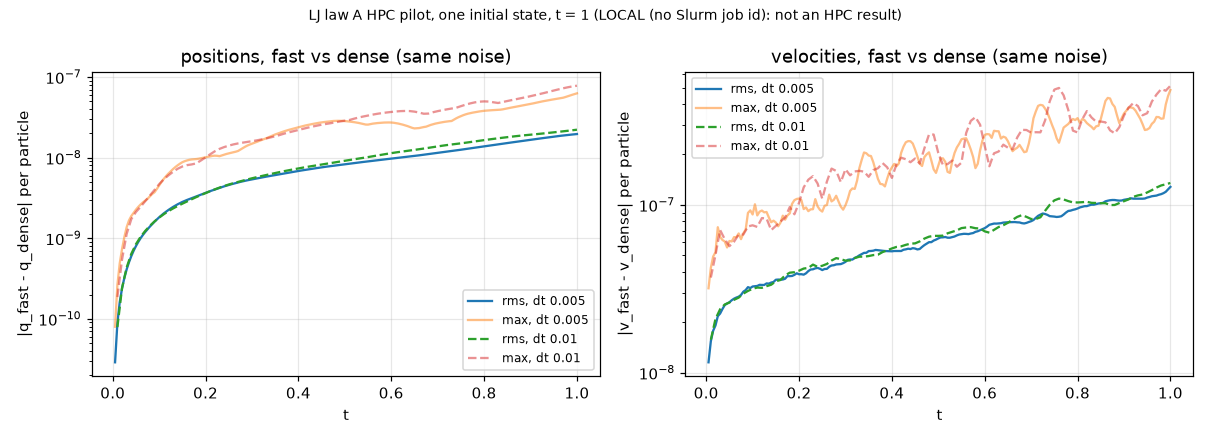
\includegraphics[width=0.49\textwidth]{pilot_fast_vs_dense.png}
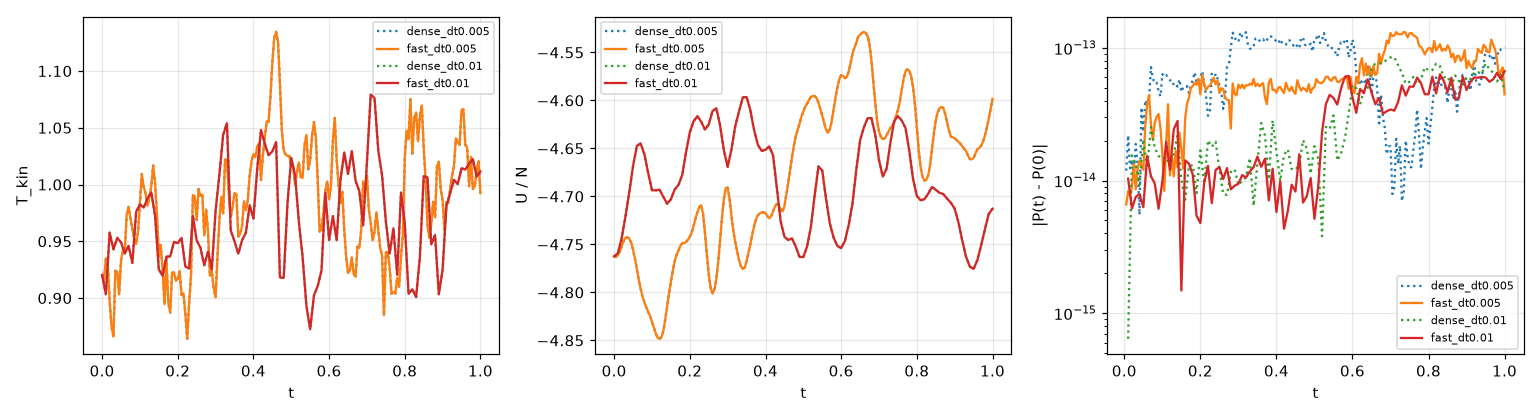
\includegraphics[width=0.49\textwidth]{pilot_diagnostics.png}
\caption{Local emulation of the HPC pilot (not run on HPC), LJ+A, $N=256$, one state, one paired noise path per dt, $t\le1$. Left:
per-particle fast$-$dense position and velocity differences (RMS and max). Right: $T_{\rm kin}$, $U/N$ and $|P(t)-P(0)|$ for the four cases.
No error bars (single path). Source: \texttt{hpc\_pilot/local\_20261010/pilot\_\{fast\_vs\_dense,diagnostics\}.png}.}
\label{fig:pilot}
\end{figure}

\clearpage
%======================================================================
\section{Historical and auxiliary evidence (not the main model)}\label{app:history}
%======================================================================

The following studies used other systems. They support the algorithmic components within their own scope and are \emph{not}
verification of the LJ+A state point. ``Config A/B'' in the Lanczos studies denotes two frozen random configurations, not the
kernels.

\begin{table}[htbp]
\centering\footnotesize
\caption{Earlier studies and their scope.}
\label{tab:history}
\begin{tabularx}{\textwidth}{>{\raggedright\arraybackslash}p{3.0cm}>{\raggedright\arraybackslash}p{3.8cm}>{\raggedright\arraybackslash}X}
\toprule
directory & system & main result (scope) \\
\midrule
\path{results/}, \path{figures/} & unit kernel, $\kappa=\xi=1$; random configs $N=30$, $L=6$ and $N=40$, $L=10$ & split error $3.6\times10^{-15}$ (scalar), $1.9\times10^{-15}$ (tensor); $\Gamma_{\rm full}$, $\Gamma_S$, $\Gamma_L$ PSD; periodic convolution with $\hat K_L$ not PSD; Fourier-truncated $\Gamma_L$ indefinite at small $k_c$ \\
\path{parameter_selection_results/} & same, $\kappa=1$ & balanced rule $\xi r_c=k_c/(2\xi)=s_\ast$; $\epsilon_S/e^{-s_\ast^2}=0.34$--$0.79$, $\epsilon_F/e^{-s_\ast^2}=0.18$--$0.44$; mesh transfer error floors accuracy near $10^{-5}$ at $\eta=0.7$, $p=4$ \\
\path{equal_accuracy_xi_results/} & same, plus $N=4000$ timing & at tolerance $10^{-7}$, one $\Gh$ action at $N=4000$: 332, 311, 532, 1366, 8145 ms for $\xi=0.5,0.7,1,1.4,2$ (machine not recorded) \\
\path{mesh_error_decomposition_results/} & $\kappa=\xi=1$, 13\,195 mesh operators & deconvolution error at round-off; alias terms 0.92--1.03 of the mesh error; slopes $p-0.1$ to $p+1.55$ (superseded by \cref{app:exp1}) \\
\path{radial_kernel_static_results/} & toy state $N=64$, $L=5.5$, $\kT=0.7$; kernels A and B & $\eop=1.27\times10^{-7}$ (LJ, A, $p=7$); $k=0$ share of $\|\Gamma\|$ 0.377; removing $k=0$ gives $\lambda_{\min}=-0.867$ \\
\path{lanczos_fdt_results/} & unit kernel $\kappa=1$, $\rho=30/216$, frozen configs; PPPM $\xi=0.7$, $s_\ast=4.1$, $\eta=0.7$, $p=7$ & median rank at $10^{-8}$: 25 (config A), 48 (config B); rank $\propto N^{0.34}$ up to $N=4000$; adaptive-tolerance cost $\propto N^{1.43}$; stopping rule $d_1\le$ tol/10 had no false stops \\
\path{lanczos_range_start_results/} & same & range start needs 1.13--1.43$\times$ more rank, 20--35\% slower; direct start adopted \\
\path{fixed_rank_budget_results/} & same, $N\le16000$ & rank 40: max error $9.1\times10^{-4}$ at $N=16000$ against a rank-360 reference (thin margin to $10^{-3}$) \\
\path{dynamics_results/} & ideal gas, $\kappa=1$, A--O--A, $N=64$--16000 & rank-40 vs dense $\le1.0\times10^{-9}$ (N=64); production step 0.79/6.35/37.4 s at $N=512$/4000/16000 (rank 40/16) \\
\path{toy_fixed_time_results/} & double well, kernel A, $N=64$, 5 states $\times$ 16 paths & fast$-$dense 95\% bounds $\le2\times10^{-5}$ \\
\path{toy_dynamics_results/} & LJ and double well, kernels A, B, $N=64$, $t=60$ & momentum $\le1.1\times10^{-12}$; unexplained seed-paired $D_{\rm GK}$ difference $+8.0\%$ $[4.1,12.0]$ (double well, A); raw trajectories absent \\
\path{cost_optimization_results/}, \path{fft_vs_direct_results/} & toy state, double well, $p=7$ sets & full-step crossover PPPM vs direct periodic sum: $108<N\le256$ (A), $64<N\le108$ (B); at $N=1728$ PPPM $\times7.9$--$9.9$ (A) faster than direct sum, $\times12$--21 than dense (2.10 GHz Xeon, 1 thread) \\
\bottomrule
\end{tabularx}
\end{table}

\begin{table}[htbp]
\centering\scriptsize
\caption{Parameters of the earlier studies (n/r: not recorded in the result files). ``Exp1'' is the newer $\kappa=1$ operator study of
\cref{app:exp1}; the LJ+A production row is repeated for contrast. Amplitudes: kernel A $c=1.615$, kernel B $0.956$, unit kernel 1.}
\label{tab:history_params}
\setlength{\tabcolsep}{3pt}
\begin{tabularx}{\textwidth}{>{\raggedright\arraybackslash}p{3.3cm}>{\raggedright\arraybackslash}p{1.4cm}>{\raggedright\arraybackslash}p{1.3cm}l>{\raggedright\arraybackslash}p{1.3cm}>{\raggedright\arraybackslash}p{1.6cm}>{\raggedright\arraybackslash}X>{\raggedright\arraybackslash}p{1.6cm}>{\raggedright\arraybackslash}p{1.4cm}}
\toprule
study & $N$ & $L$ / density & $\kT$ & potential & kernel, $\kappa$ & PPPM $\xi$ / $s_\ast$ / $\eta$ / $p$ & rank (n/d) & machine \\
\midrule
\path{results/}, \path{parameter_selection_results/} & 30, 40 (4000 timing) & $L=6$, 10 (30) & -- & static & unit, 1 & $\xi=1$ (scan 0.5--2), $s_\ast$ 2.5--5, $\eta$ 0.3--0.8, $p$ 2--8 & dense & n/r \\
\path{equal_accuracy_xi_results/} & 30, 40, 4000 & as above & -- & static & unit, 1 & $\xi$ 0.5--2, per-tolerance search & -- & n/r \\
\path{mesh_error_decomposition_results/} & 30, 40 & $L=6$, 10 & -- & static & unit, 1 & $\xi=1$, $k_c$ 4/6, $p$ 2--8 & -- & n/r \\
\path{radial_kernel_static_results/} & 64 & $L=5.5$ & 0.7 & LJ, DW, uniform & A, B; 0.7 & 0.7 / 4.1 / 0.7 / 7 ($M=15$) & 40/16 & n/r \\
\path{lanczos_fdt_results/}, \path{lanczos_range_start_results/}, \path{fixed_rank_budget_results/} & 128--16000 & $\rho=30/216$ & 1 & frozen random & unit, 1 & 0.7 / 4.1 / 0.7 / 7 & adaptive; 16--48 & n/r \\
\path{dynamics_results/} & 64--16000 & $\rho=30/216$ & 1 & ideal gas & unit, 1 & 0.7 / 4.1 / 0.7 / 7 & 40/12, 48/16 & 1 thread, CPU n/r \\
\path{toy_fixed_time_results/}, \path{toy_dynamics_results/} & 64 & $L=5.5$ & 0.7 & DW; LJ and DW & A (and B); 0.7 & 0.7 / 4.1 / 0.7 / 7 & 40/16 & n/r \\
\path{cost_optimization_results/} & 64--4096 & $64/5.5^3$ & 0.7 & DW & A, B; 0.7 & A at $2\times10^{-7}$: 0.85 / 4.1 / 0.678 / 7 & 32/4 (A) & Xeon 2.30\,GHz, 1 thread \\
\path{fft_vs_direct_results/} & 64--1728 & $64/5.5^3$ & 0.7 & DW & A, B; 0.7 & high-accuracy sets of the cost study & 32/5--64/5 (A) & Xeon 2.10\,GHz, 1 thread \\
Exp1 (\path{exp1_results/}) & 30--256 & see \cref{tab:exp1_configs} & -- & static & unit, 1 & T5/T7/T9, \cref{tab:exp1_params} & dense & host ``vm'', 1 thread \\
law B at LJ point & 256 & $\rho^*=0.75$ & 1 & LJ & B; 0.7 & 1.0 / 3.9 / 0.683 / 7 & -- & host ``vm'' \\
\midrule
LJ+A production & 256 & $\rho^*=0.75$ & 1 & LJ & A; 0.7 & 0.85 / 4.1 / 0.6779 / 8 ($M=24$) & 12/5 used, 14/5 rec. & host ``vm'' \\
\bottomrule
\end{tabularx}
\end{table}

\begin{figure}[htbp]
\centering
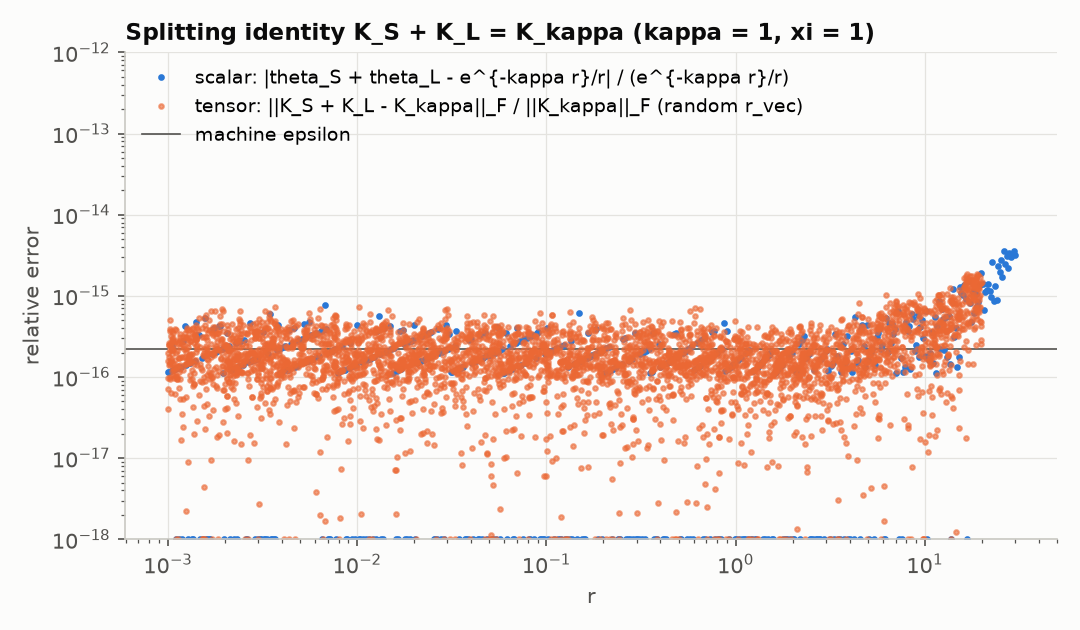
\includegraphics[width=0.45\textwidth]{hist_kappa1_splitting.png}
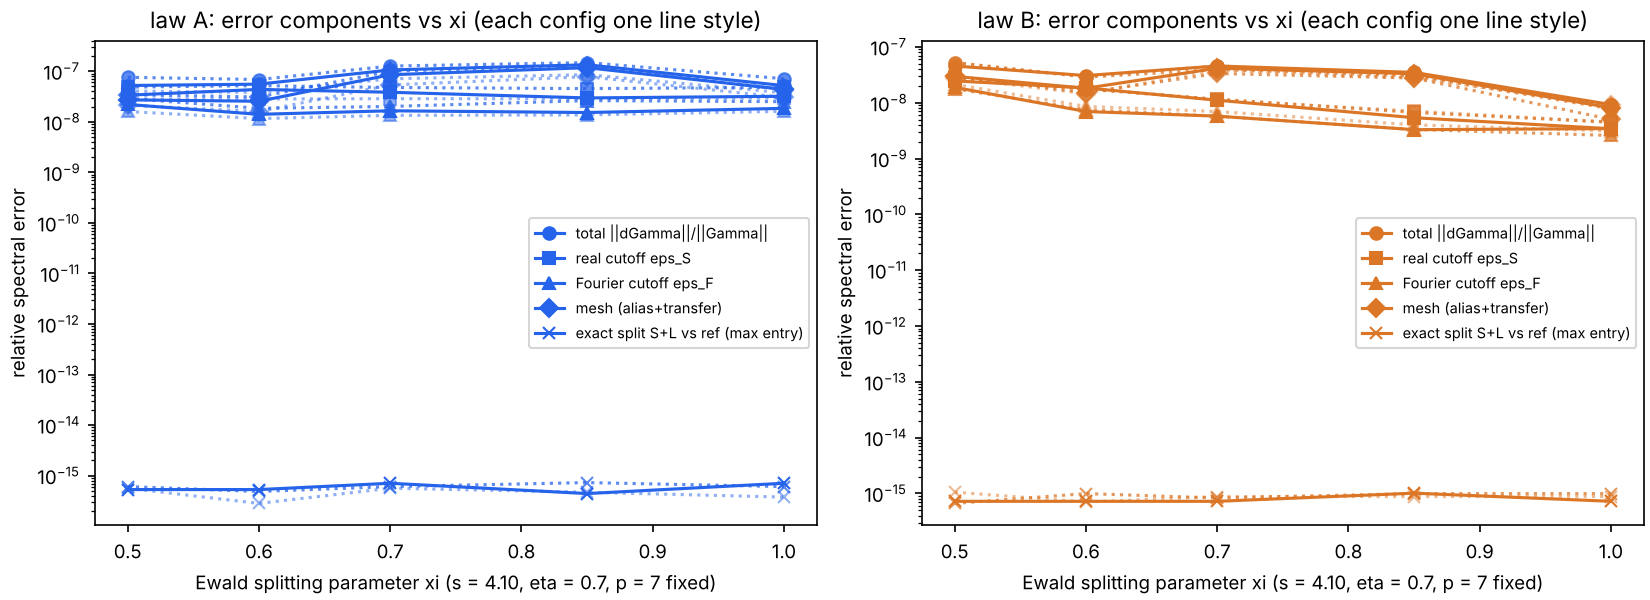
\includegraphics[width=0.53\textwidth]{hist_toy_error_budget_xi.png}\\
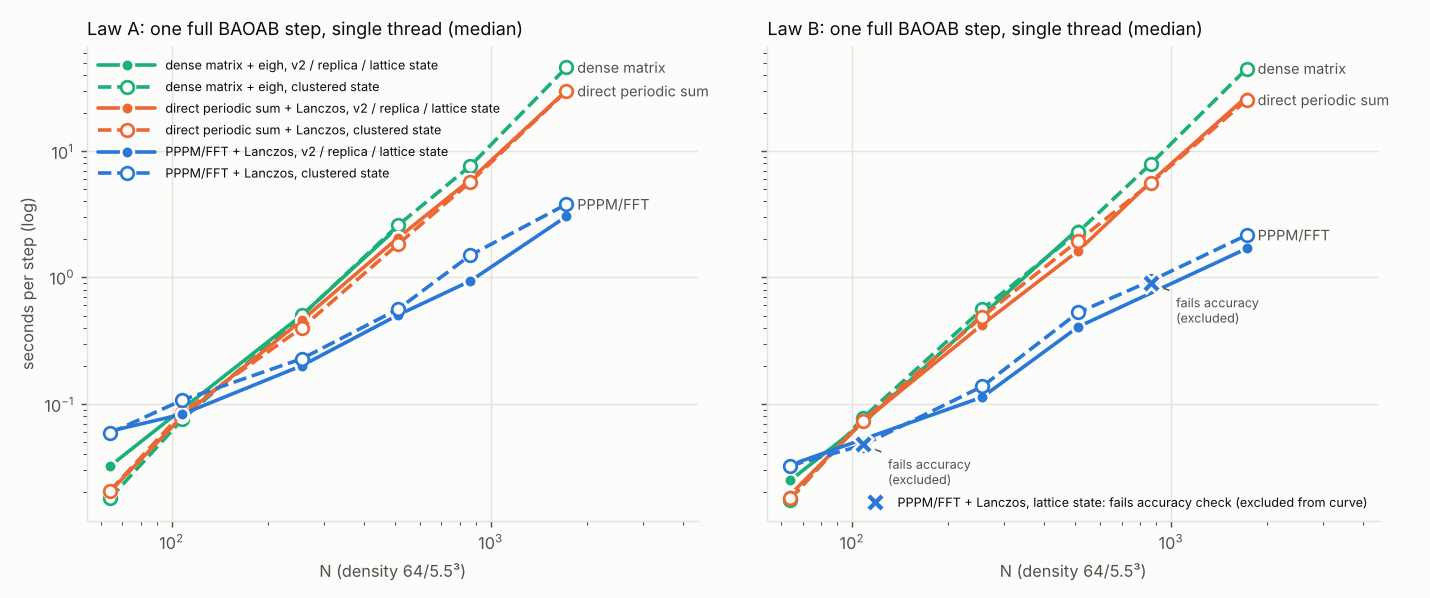
\includegraphics[width=0.9\textwidth]{hist_toy_step_time_vs_N.png}\\
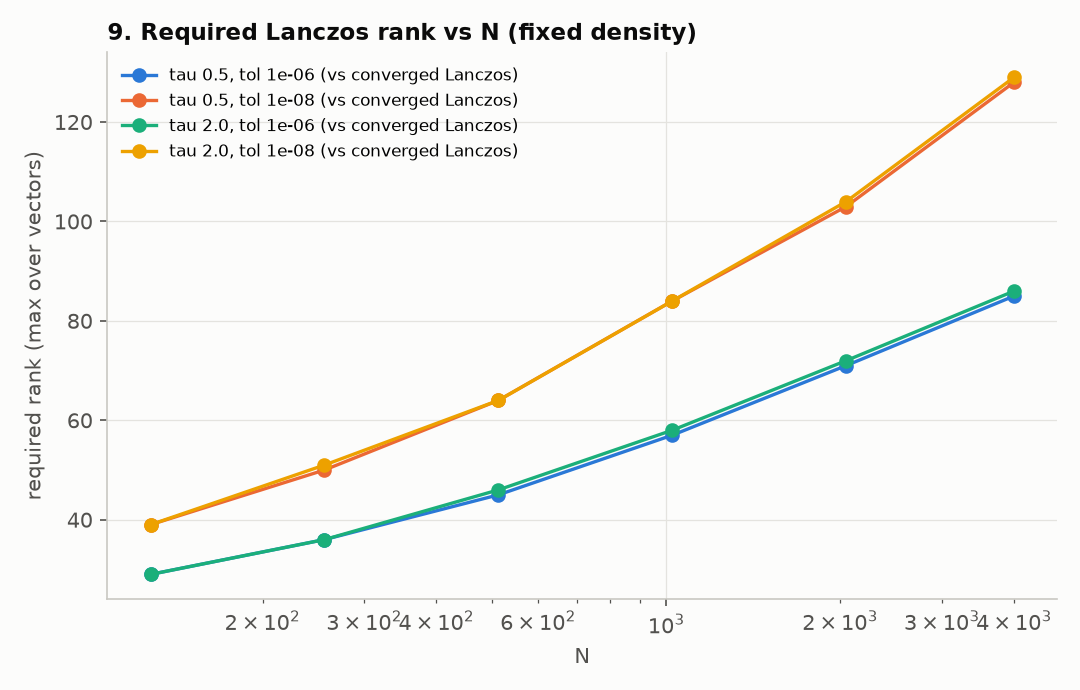
\includegraphics[width=0.5\textwidth]{hist_lanczos_rank_vs_N.png}
\caption{Historical evidence, \emph{not} at the LJ+A state point. Top left: Ewald splitting error, unit kernel $\kappa=\xi=1$
(\texttt{figures/fig1\_splitting\_error.png}). Top right: PPPM error budget versus $\xi$ at the toy state ($N=64$, $L=5.5$, $\kT=0.7$;
\texttt{radial\_kernel\_static\_results/fig1\_error\_budget\_vs\_xi.png}). Middle: full BAOAB step time versus $N$ at the toy density
$64/5.5^3$ with double-well forces: dense matrix + eigendecomposition, direct periodic sum + Lanczos, PPPM + Lanczos; single thread,
median; points failing the accuracy check are excluded (\texttt{fft\_vs\_direct\_results/step\_time\_vs\_N.png}). Bottom: required Lanczos
rank versus $N$ for the unit kernel at $\rho=30/216$ (\texttt{lanczos\_fdt\_results/plot09\_rank\_vs\_N.png}).}
\label{fig:history}
\end{figure}

\subsection{Kernel B (stopped)}\label{app:lawB}
Law B, $g(r)=c_Br\,e^{-\kappa r}$ with $c_B=\gamma e^{\kappa r_{\rm ref}}/r_{\rm ref}$, has Gaussian-scale weight $w_\kappa$ instead of
$\rho_\kappa$. At the LJ state point it was verified statically on 42 states ($\eop\le2.4\times10^{-8}$ full norm, $1.4\times10^{-7}$
relative to the $k\neq0$ part, which exceeds its $5\times10^{-8}$ budget under that definition; a tighter set passes both). The campaign
was stopped at the user's request; dynamic runs exist only as raw data and were not analysed.

\clearpage
\subsection{Operator-level verification on the unit kernel (Experiment 1, $\kappa=1$)}\label{app:exp1}

This study is the most recent and most complete check of the spatial operator, but it is \emph{not} at the LJ+A state
point: the kernel is the unit-amplitude $K_\kappa$ with $\kappa=1$, the configurations are static and synthetic, and the
PPPM sets use $\xi=0.7$ (\cref{tab:exp1_params}), not the production set of \cref{sec:setup}. It supersedes the $\kappa=1$
operator checks in \path{results/}, \path{parameter_selection_results/} and \path{mesh_error_decomposition_results/} as
evidence for the error components of \cref{sec:errors}. Source: \path{exp1_results/} (\texttt{summary.json} and CSV files),
scripts \texttt{exp1\_operator\_action.py}, \texttt{exp1\_plots.py}; at the time of writing these exist only on the remote
branch (commits \texttt{7b8049f}--\texttt{dce9792}).

\paragraph{Configurations and reference.}
\Cref{tab:exp1_configs} lists the 44 configurations: the two original test boxes (A, B), three families at $N=128$ and
$N=256$ at the density $n_A=30/216$ of case A (uniform, perturbed bcc/fcc lattice, clustered), and two box-length sets.
$\Gref$ is the unsplit periodic lattice sum over images $|\br_{ij}+\bn L|\le R$, with nothing removed (so $k=0$ is included).
Increasing $R$ from 15 to 45, the largest change relative to $R=45$ is $2.5\times10^{-12}$ at $R=30$, $2.0\times10^{-14}$ at
$R=35$ and $4.3\times10^{-16}$ at $R=40$ (spectral norm relative to $\|\Gref\|_2$); $R=45$ is used.

\begin{table}[htbp]
\centering\small
\caption{Static configurations of Experiment 1 ($\kappa=1$, so $L=\kappa L$). $n=N/L^3$; $d_{\min}$ is the smallest periodic pair
distance (range over seeds). Source: \texttt{exp1\_results/configs.csv}.}
\label{tab:exp1_configs}
\begin{tabular}{llrlllr}
\toprule
set & generation & $N$ & $L$ & $n$ & $d_{\min}$ & seeds \\
\midrule
A & uniform, seed 7 & 30 & 6 & 0.139 & 0.395 & 1 \\
B & uniform, seed 13 & 40 & 10 & 0.040 & 0.589 & 1 \\
U128 & uniform i.i.d. & 128 & 9.73 & 0.139 & 0.142--0.411 & 3 \\
L128 & bcc $4^3$, $\sigma=0.1\,d_{\rm nn}$ & 128 & 9.73 & 0.139 & 1.208--1.366 & 3 \\
C128 & clusters of 16, $\sigma_c=0.5$, $d\ge0.25$ & 128 & 9.73 & 0.139 & 0.251--0.255 & 3 \\
U256 & uniform i.i.d. & 256 & 12.3 & 0.139 & 0.148 & 1 \\
L256 & fcc $4^3$, $\sigma=0.1\,d_{\rm nn}$ & 256 & 12.3 & 0.139 & 1.011 & 1 \\
C256 & clusters of 16, $\sigma_c=0.5$, $d\ge0.25$ & 256 & 12.3 & 0.139 & 0.259 & 1 \\
box-$N$ & uniform i.i.d. & 64 & 4--16 (6 values) & 0.016--1.00 & 0.090--0.723 & 3 \\
box-$n$ & uniform i.i.d. & 30--240 & 6--12 (4 values) & 0.139 & 0.055--0.924 & 3 \\
\bottomrule
\end{tabular}
\end{table}

\begin{table}[htbp]
\centering\small
\caption{PPPM sets of Experiment 1, accepted at $\xi=0.7$ for relative tolerances $10^{-5}$, $10^{-7}$, $10^{-9}$ on cases A and B.
$M$ is the next $2,3,5$-smooth mesh size with $h\le\eta_N\pi/k_c$. Source: \texttt{exp1\_results/action.csv}.}
\label{tab:exp1_params}
\begin{tabular}{lllllll}
\toprule
set & $\xi$ & $s_\ast$ & $r_c$ & $k_c$ & $\eta_N$, $p$ & $M$ (A / B / $N\!=\!128$ / $N\!=\!256$) \\
\midrule
T5 & 0.7 & 3.494 & 4.991 & 4.891 & 0.8, 6 & 12 / 20 / 20 / 24 \\
T7 & 0.7 & 4.100 & 5.857 & 5.740 & 0.7, 7 & 16 / 27 / 27 / 36 \\
T9 & 0.7 & 4.628 & 6.611 & 6.479 & 0.6, 8 & 24 / 36 / 36 / 45 \\
\bottomrule
\end{tabular}
\end{table}

\paragraph{Error components, each measured alone.}
(i) \emph{Split identity.} With $\theta_S$ in closed form and $\theta_L$ from its own $s$-integral, $\theta_S+\theta_L=e^{-\kappa r}/r$
holds to $2.5\times10^{-15}$ for $\xi\in\{0.5,0.7,1,1.4,2\}$; at operator level, $\Gamma_S$ (real-space lattice sum) plus the
mesh-free Fourier lattice sum of $\hat K_L$ (including $\bk=0$) reproduces $\Gref$ to $6.7\times10^{-15}$--$2.2\times10^{-13}$, a floor
of the float64 Fourier lattice sum that is unchanged by 80-bit accumulation or refined quadrature of $A,B$.
(ii) \emph{Truncation.} Fitting $\log E=a-cx^2$ with $x=\xi r_c$ or $k_c/(2\xi)$ gives median rates $c=0.99$ (real space, range
$0.98$--$1.03$) and $0.97$ (Fourier, $0.96$--$1.00$) at $\xi=0.7$ and $\xi=1$, consistent with the $e^{-s_\ast^2}$ balance
of~\eqref{eq:balance}; the algebraic prefactor of the operator-norm error is not that of the continuum tail.
(iii) \emph{Mesh.} Against the mesh-free sum over the same modes, the mesh error decays as $h^p$ on $\eta\approx0.23$--$0.50$ (median
fitted slopes $3.09$, $4.07$, $5.24$, $6.19$, $7.46$, $8.50$ for $p=3,\dots,8$) and faster on coarser meshes ($1.1$--$1.3\,p$); the
asymptotic constant is not reached. Over eight random grid shifts the maximum error is at most $1.30$ times the RMS. In an exact
alias decomposition the linear cross terms between the principal term and the aliases carry $0.996$--$1.003$ of the mesh error and the
alias--alias term at most $0.9\%$; the deconvolution error vanishes to $5\times10^{-9}$ of it.

\paragraph{The complete production action.}
Applying the production spread--FFT--influence--gather code with the degree correction to the $3N$ unit vectors gives $\Gh$ column by
column; it agrees with an independent mode-space assembly to $1.1\times10^{-15}$, so $\varepsilon_S$, $\varepsilon_F$ and
$\varepsilon_{\rm mesh}$ telescope to the production error. Cases A and B meet their tolerances, as selected; uniform and clustered
configurations at $N=128$, 256 meet them with margin; the perturbed lattices exceed them by up to a factor $2.5$ (T7:
$1.94$--$2.11\times10^{-7}$ at $N=128$). The reason is the normalisation: at T7 the absolute error $\|\Gh-\Gref\|_2$ lies in
$5.7\times10^{-8}$--$5.5\times10^{-7}$ over all 44 configurations, whereas $\|\Gref\|_2$ ranges over $0.72$--$35$, set by the closest pair.
A tolerance relative to $\|\Gref\|_2$ calibrated on configurations with close pairs therefore does not transfer to configurations
without them. Probe vectors at the lowest wave number $2\pi/L$ have relative action errors up to $14$ (longitudinal) and $18$
(transverse) times the configuration's relative spectral error, because $\|\Gref X\|/(\|\Gref\|_2\|X\|)$ is small for such modes.
$\Gh T_\alpha=0$ exactly in floating point, $\Gh$ is symmetric to $1.0\times10^{-16}$, and $\|\Gh-\Gref\|_2<\lambda_{\min}(\Gref|_{\Ran\Pi})$ in
every case.

\paragraph{Relevance for LJ+A.}
The configuration dependence of the relative error is consistent with what was observed at the LJ+A point, where the $p=7$ set inherited
from the toy state failed the budget on fcc-lattice states (\cref{sec:setup}); for this reason the LJ+A operator was verified on its own
representative and visited states (\cref{sec:numerics_space}) rather than on transferred calibrations. Experiment 1 was not repeated at
$\kappa=0.7$ with the production set.

\begin{figure}[htbp]
\centering
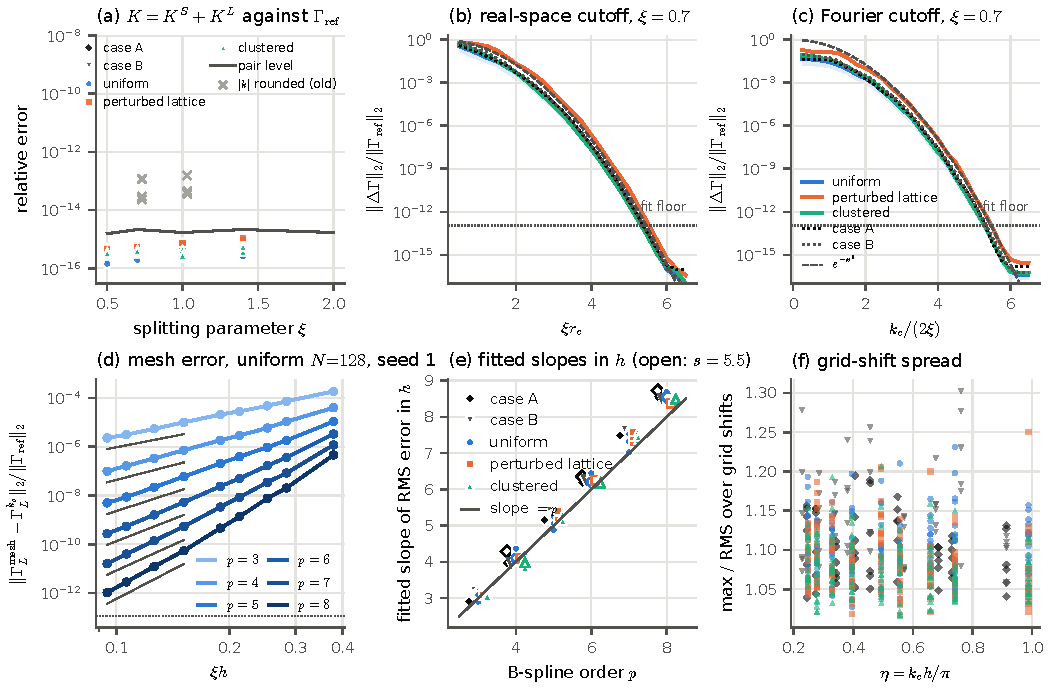
\includegraphics[width=\textwidth]{exp1_components.pdf}
\caption{Experiment 1 ($\kappa=1$, unit amplitude, static configurations of \cref{tab:exp1_configs}; \emph{not} LJ+A). (a) Split identity at
operator level against $\Gref$; line: pair-level error. (b) Real-space and (c) Fourier truncation at $\xi=0.7$ alone; curves: median over
three seeds, bands: range over seeds; dotted: cases A, B; dashed: $e^{-x^2}$. (d) Mesh error against the mesh-free sum over the same modes,
$k_c=5.74$, uniform $N=128$ seed 1; curves: RMS over eight grid shifts, bands: range over shifts. (e) Fitted slopes in $h$ (filled:
$s_\ast=4.1$; open: $s_\ast=5.5$, five configurations). (f) Max over RMS error across eight grid shifts. Source:
\texttt{exp1\_results/figures/exp1\_components.pdf} (commit \texttt{dce9792}).}
\label{fig:exp1_components}
\end{figure}

\begin{figure}[htbp]
\centering
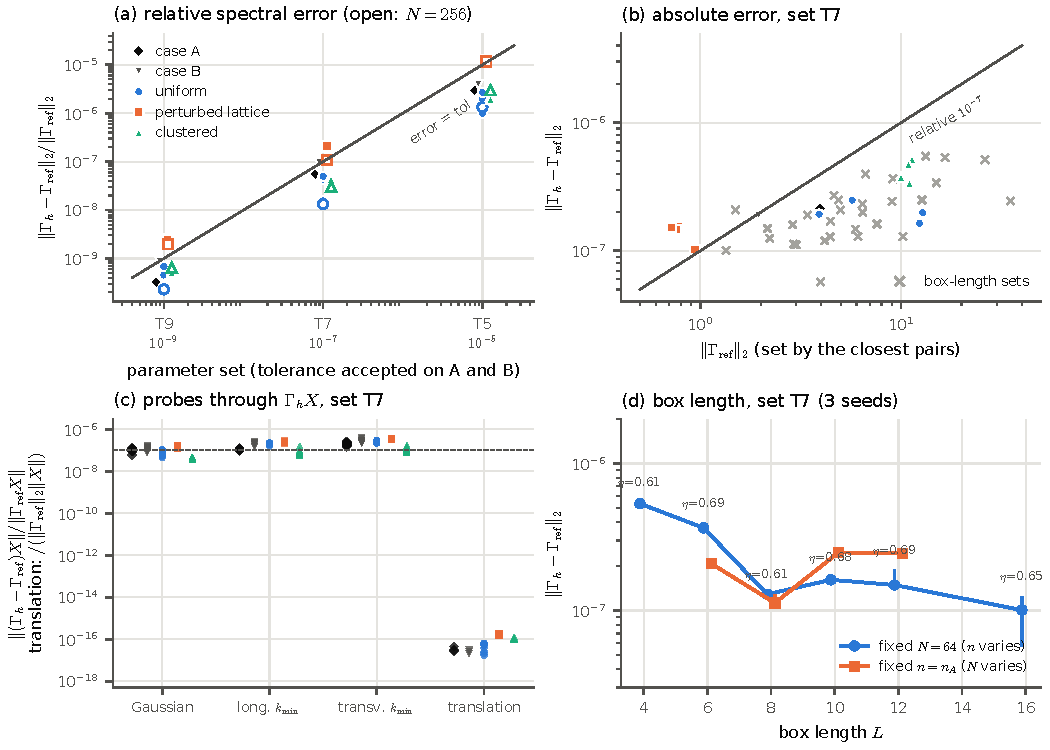
\includegraphics[width=\textwidth]{exp1_action.pdf}
\caption{Experiment 1: the production action $X\mapsto\Gh X$ against the unsplit full-periodic reference, $\kappa=1$, 44 static configurations;
one point per configuration, no error bars. (a) Relative spectral error for T9, T7, T5 (filled: $N\le128$; open: $N=256$). (b) Absolute error
against $\|\Gref\|_2$ at T7; diagonal: relative $10^{-7}$. (c) Probe errors at T7 through the production matvec; translations as
operator-normalised residuals. (d) Absolute error against box length at T7, fixed $N=64$ (density varies) and fixed density $n_A$; realised $\eta$
annotated. Source: \texttt{exp1\_results/figures/exp1\_action.pdf} (commit \texttt{dce9792}).}
\label{fig:exp1_action}
\end{figure}

\clearpage
\bibliographystyle{unsrtnat}
\bibliography{references}

\end{document}
